\section{Introduction}
In order for our estimation to work we need to collect two different types of data for our calculations. 
One is the true geometric dimension of our phantom, the other is the corresponding distorted signal that
represent those known geometric locations inside MR images. Some of these data can be relied on manufacture's
measurement, while others would require us to extract information from various types of images to estimate the
measurements. In this chapter we will discuss how we obtain each measurements and algorithm involved in those
processes.

\section{Tubes}
\label{tubes}

\section{Water Tank}
\label{ct_tank}

\subsection{CT Scan overview, target surfaces}
Due to the limitation of manufacture equipments, water tank at each end can only be guaranteed that their
surfaces are parallel \footnote{what's the error?} to each other, their accurate distances betweeen each other
are unknown. We decided to perform a CT scan\footnote{what's the CT's error} on the phantom, then collect each
surfaces' data points through coronal view CT images. With enough data points on each surface, we should be
able to have a good estimation of the distances with between each pair of surfaces. \footnote{brief outline of full algorithm}

\begin{figure}[htb]
  \begin{minipage}[t]{2.75in}
    \centering
    \centerline{\mbox{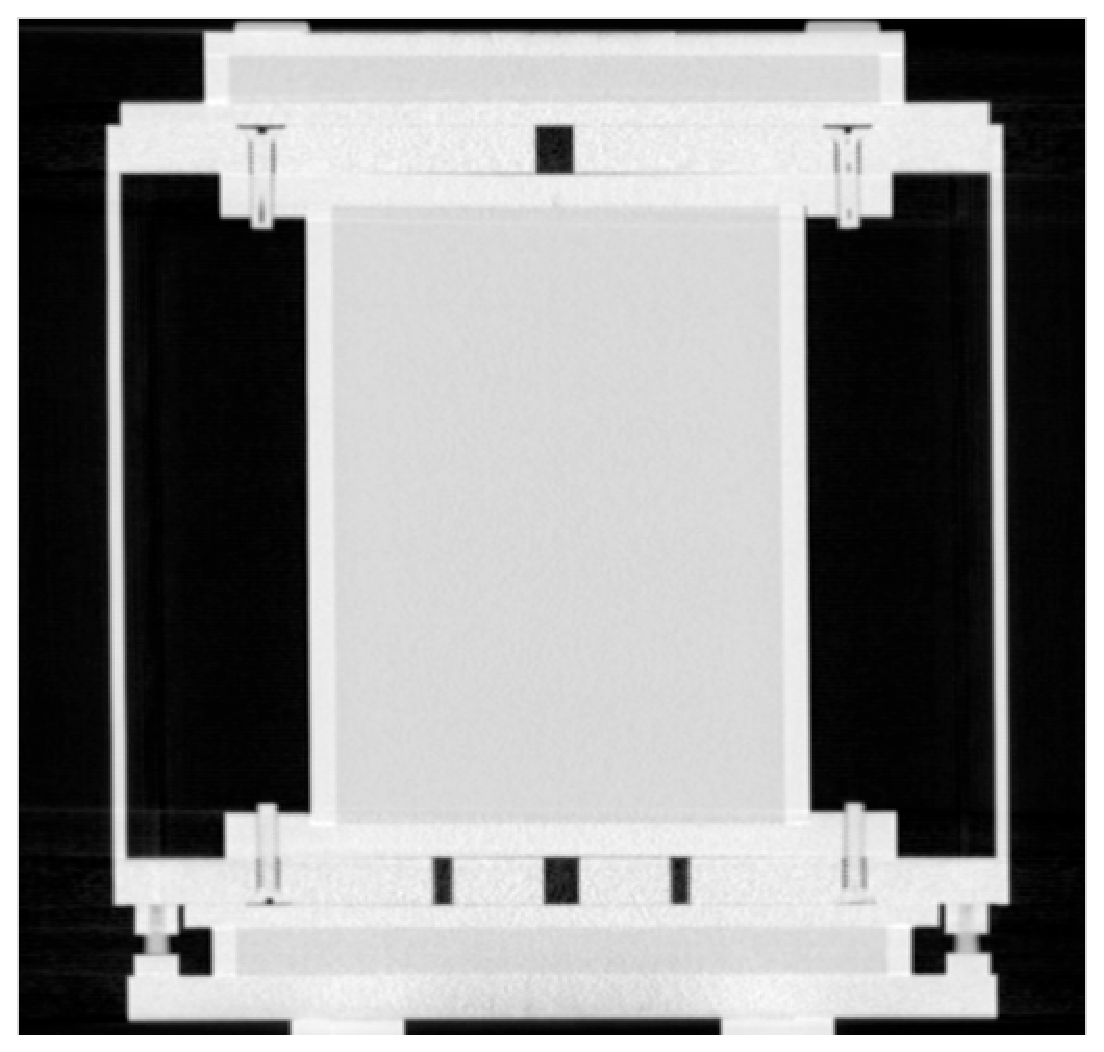
\includegraphics[width=2.75in]{data_extraction/images/targets/ct_coronal_mid_slice.eps}}}
    \centerline{\emph{(a) Coronal view, center slice}}
  \end{minipage}\medskip
  \begin{minipage}[t]{2.75in}
    \centering
    \centerline{\mbox{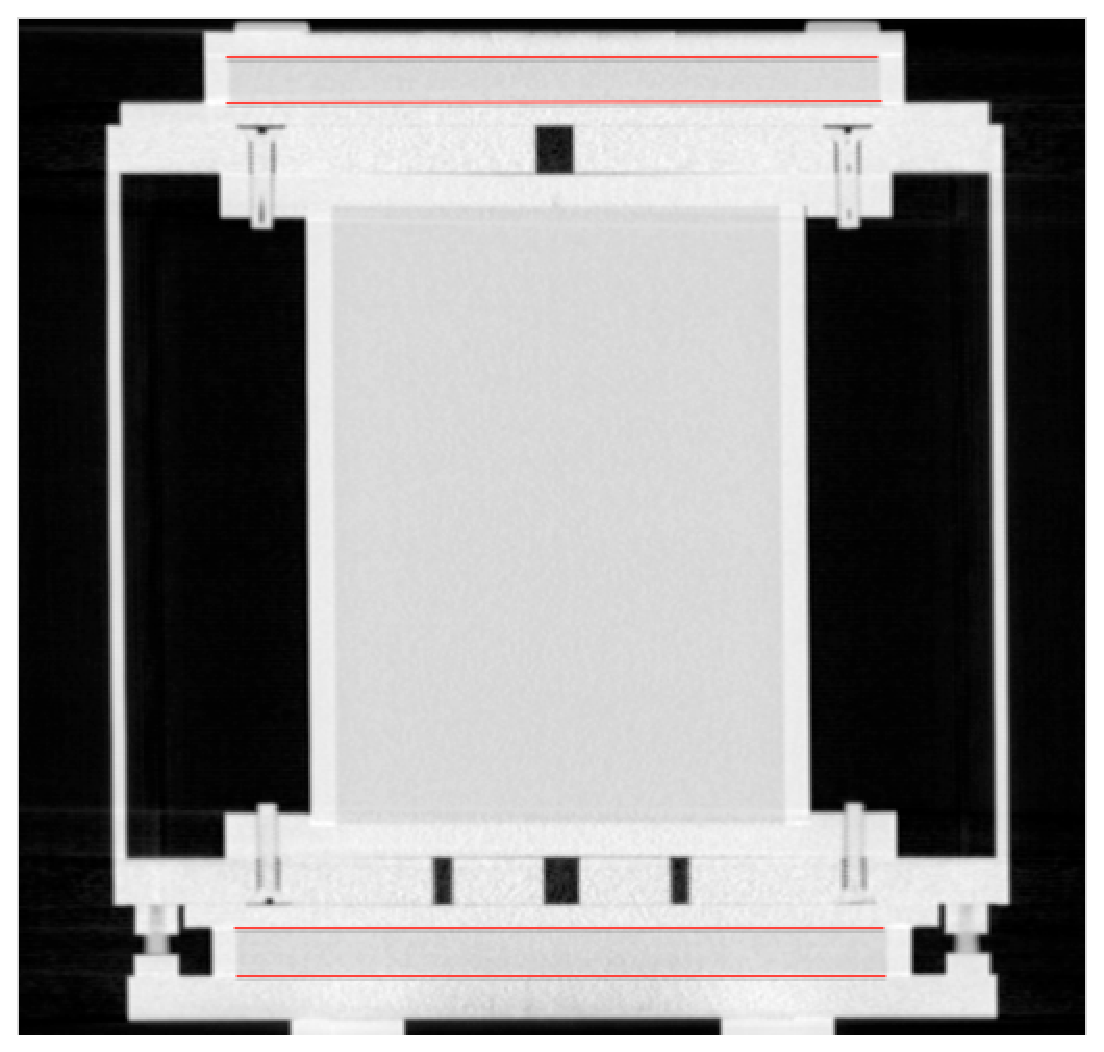
\includegraphics[width=2.75in]{data_extraction/images/targets/ct_coronal_mid_slice_marked_surface.eps}}}
    \centerline{\emph{(b) Marked target surfaces}}
  \end{minipage}
\end{figure}

Above images indicates the target feature we are looking for inside a typical coronal view of CT image.

\subsection{Canny Edges}

The obvious method is to extract the data points is to apply an edge detection algorithm on the image, then
iterate through the resulting edge image to collection the desired lines. However, the resulting edge image from
this approach often contain fair amount of noise edges some of which overlap with the desired edges we are looking
for. This problem is illustrated in figure \ref{fig:canny_ct_141}, \ref{fig:canny_ct_270} and \ref{fig:canny_ct_276}.
 
\begin{figure}[htb]
  \begin{minipage}[t]{2.75in}
    \centering
    \centerline{\mbox{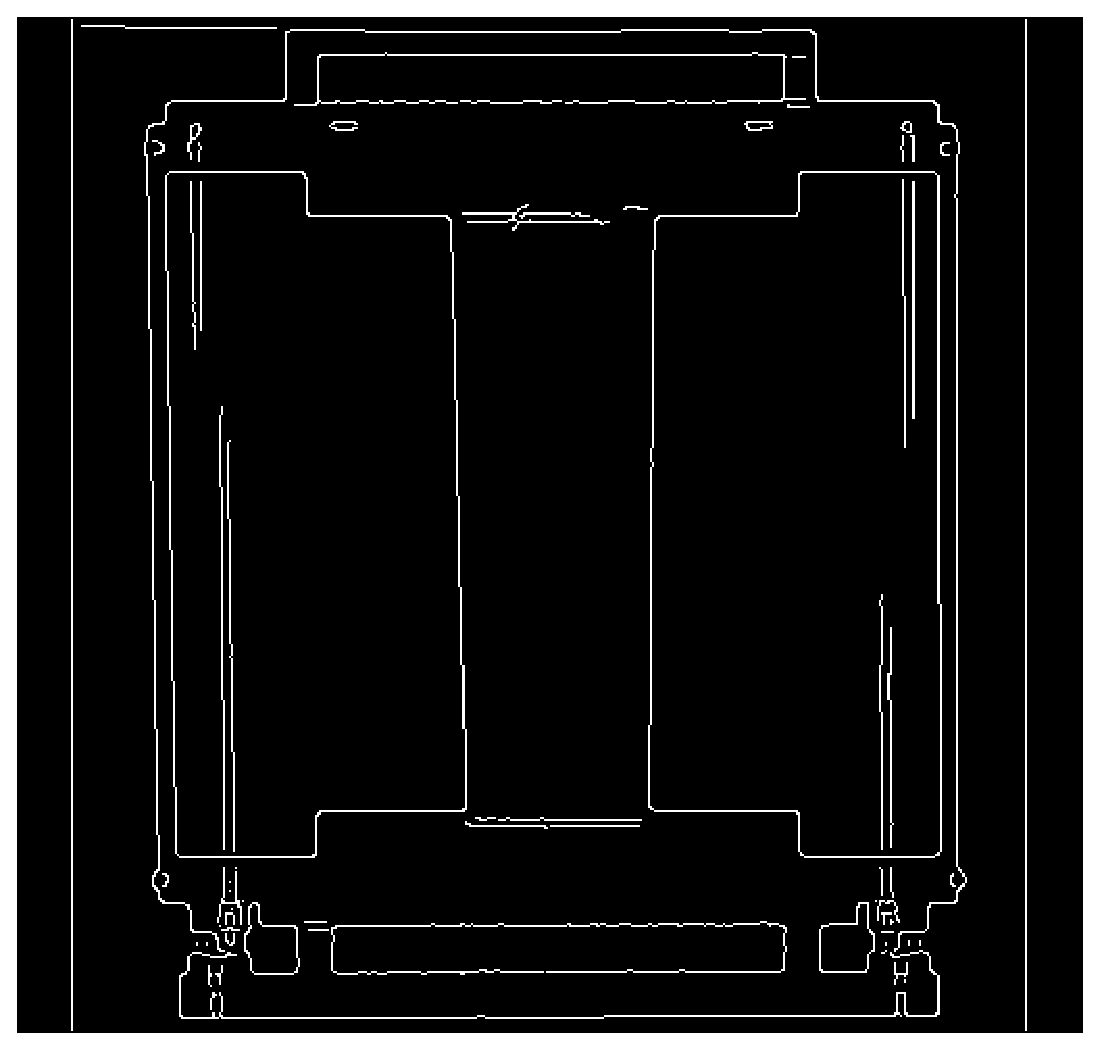
\includegraphics[width=2.75in]{data_extraction/images/canny/default/20121017_141.eps}}}
    \centerline{\emph{(a) Default parameters}}
  \end{minipage}\medskip
  \begin{minipage}[t]{2.75in}
    \centering
    \centerline{\mbox{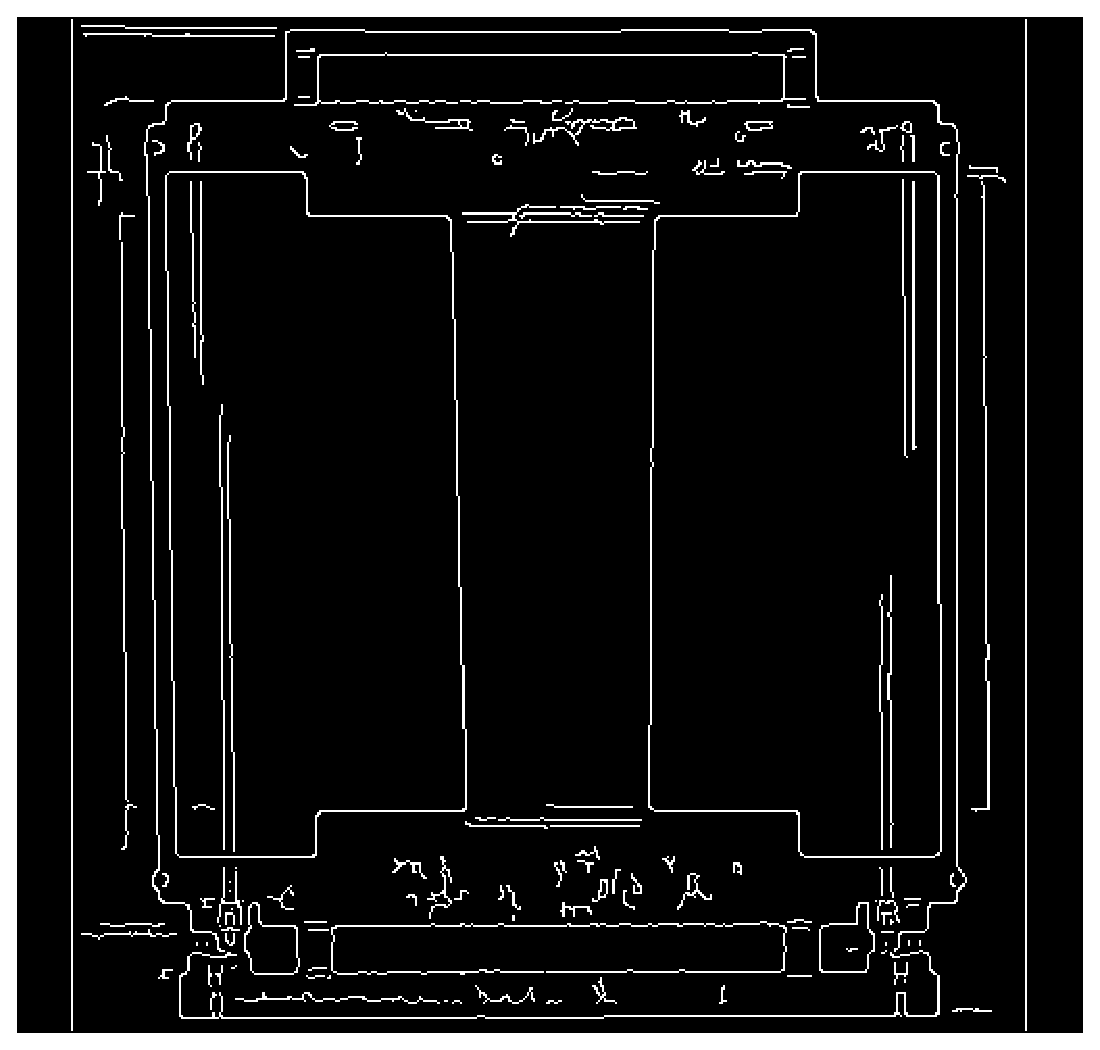
\includegraphics[width=2.75in]{data_extraction/images/canny/0.01_0.02/20121017_141.eps}}}
    \centerline{\emph{(b) Low threshold 0.01, high threshold  0.02}}
  \end{minipage}
  \begin{minipage}[t]{2.75in}
    \centering
    \centerline{\mbox{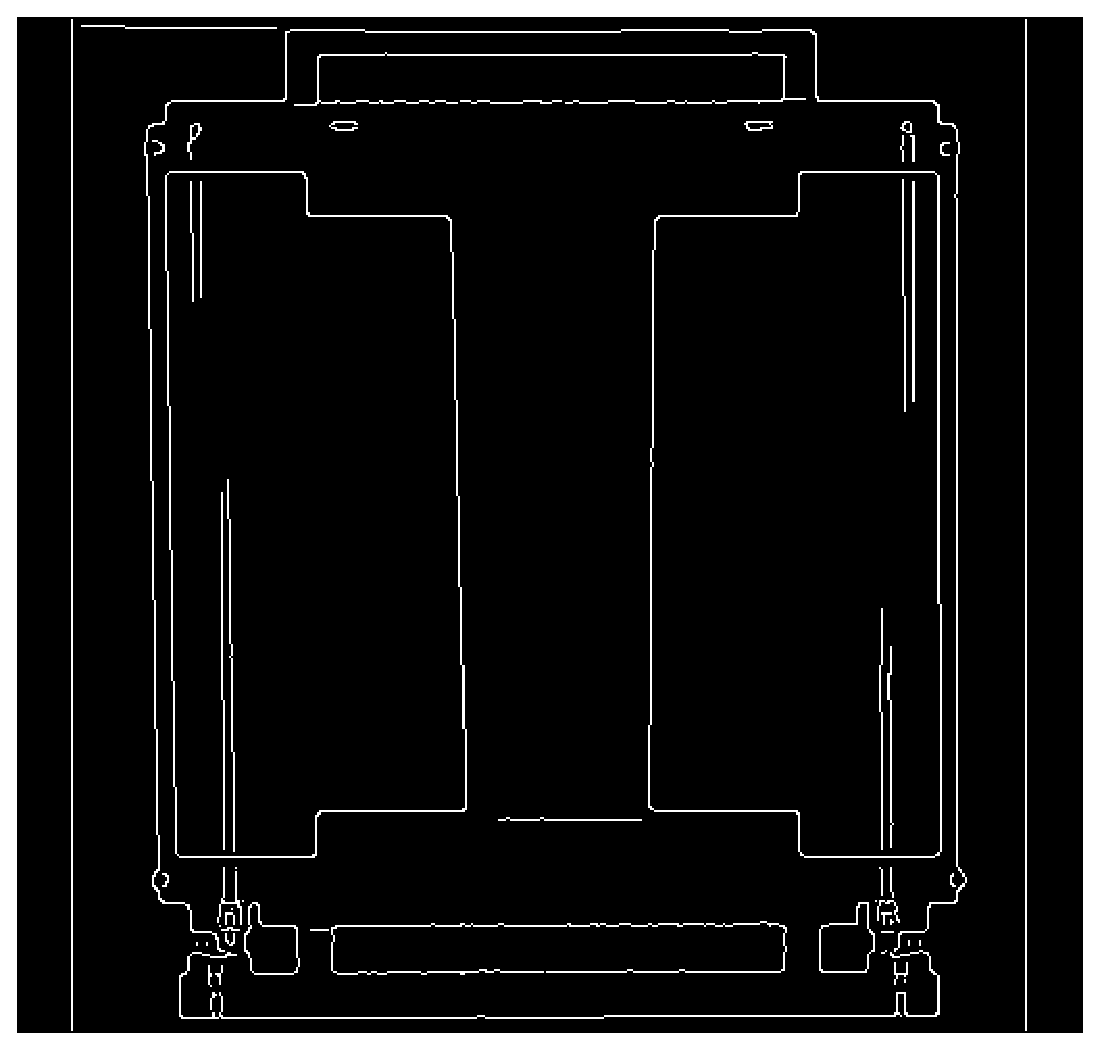
\includegraphics[width=2.75in]{data_extraction/images/canny/0.02_0.04/20121017_141.eps}}}
    \centerline{\emph{(c) Low threshold 0.02, high threshold  0.04}}
  \end{minipage}\medskip
  \begin{minipage}[t]{2.75in}
    \centering
    \centerline{\mbox{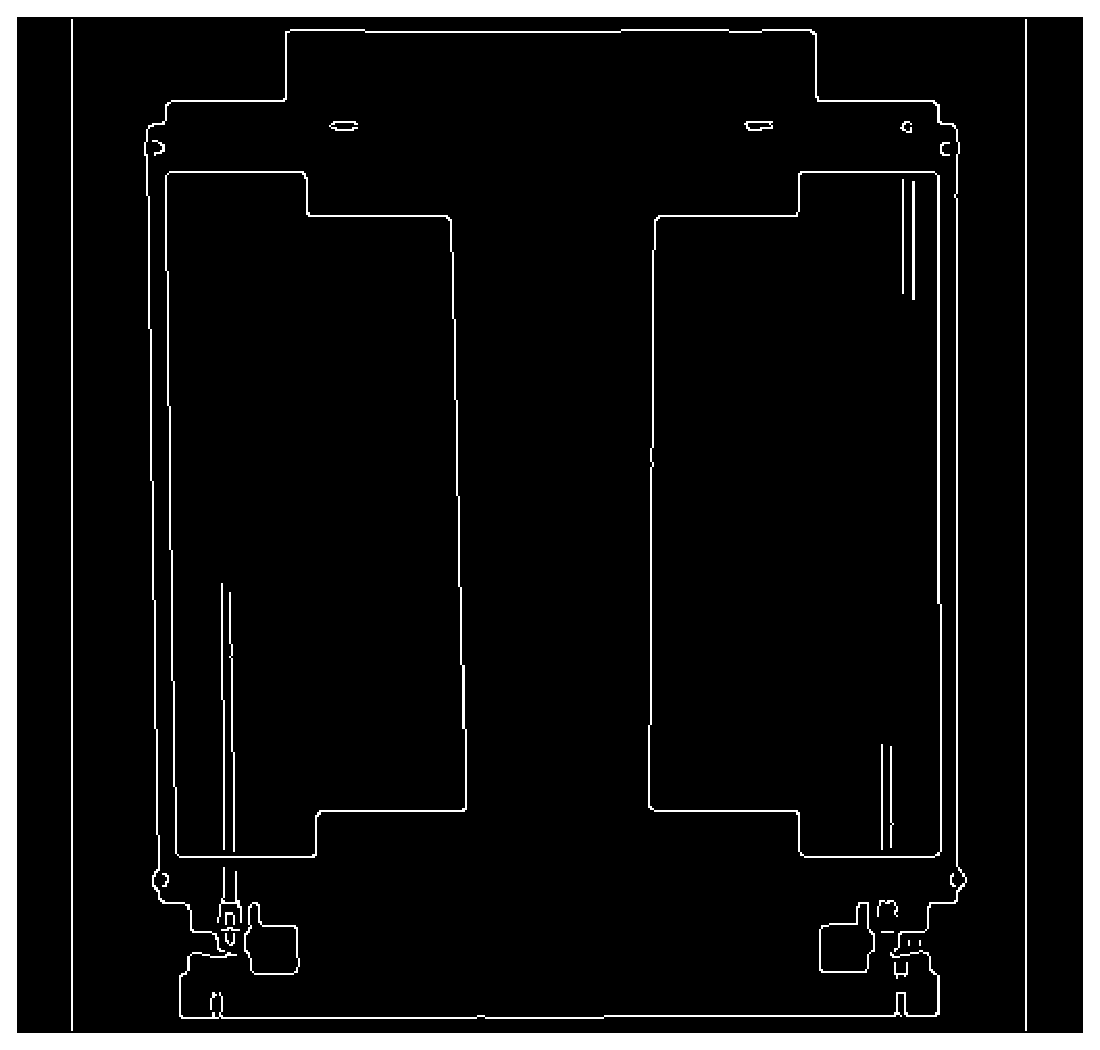
\includegraphics[width=2.75in]{data_extraction/images/canny/0.05_0.1/20121017_141.eps}}}
    \centerline{\emph{(d) Low threshold 0.05, high threshold  0.1}}
  \end{minipage}
  \caption{\emph{Canny algorithm applied to coronal sequence 141 with different parameters}} \label{fig:canny_ct_141}
\end{figure}


\begin{figure}[htb]
  \begin{minipage}[t]{2.75in}
    \centering
    \centerline{\mbox{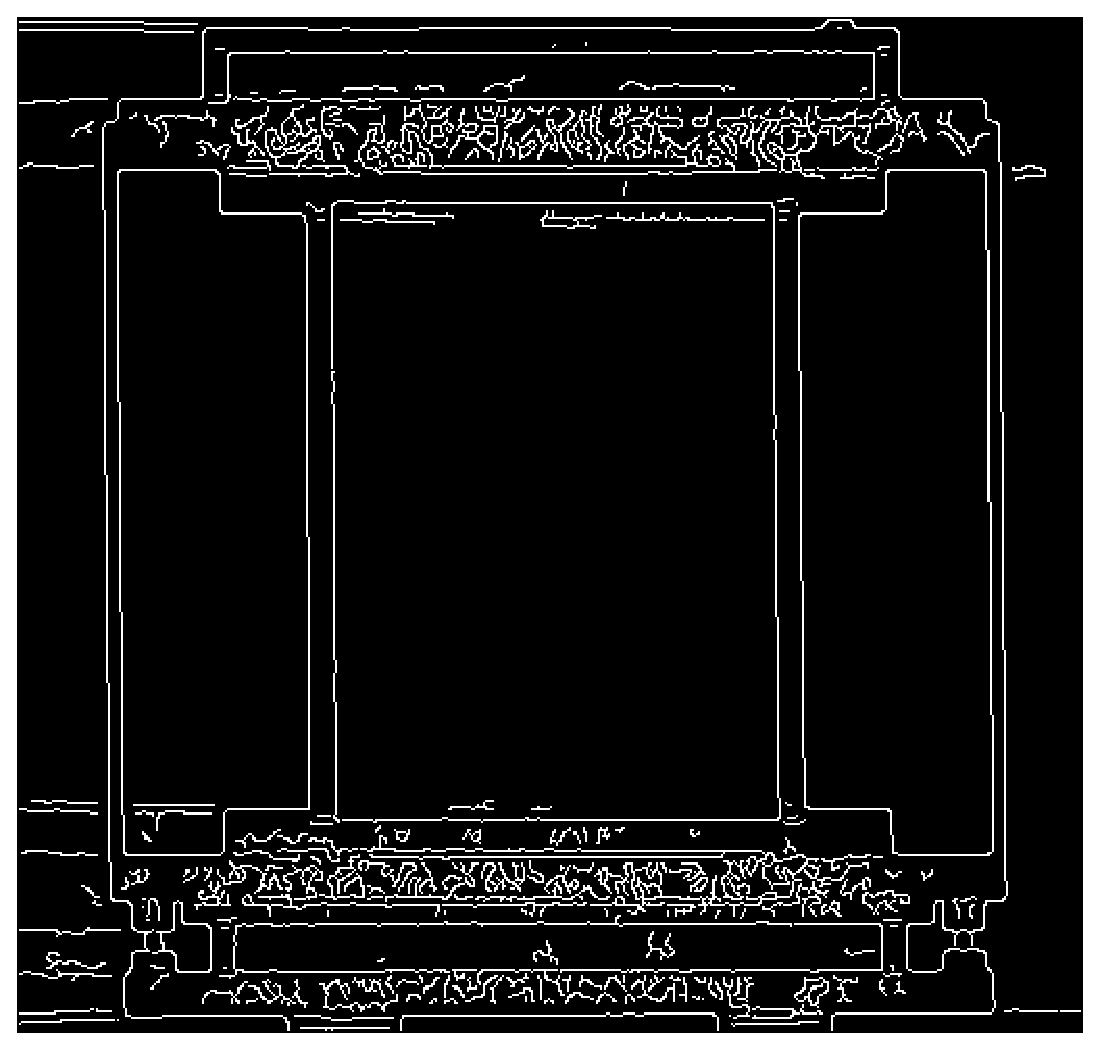
\includegraphics[width=2.75in]{data_extraction/images/canny/default/20121017_270.eps}}}
    \centerline{\emph{(a) Default parameter}}
  \end{minipage}\medskip
  \begin{minipage}[t]{2.75in}
    \centering
    \centerline{\mbox{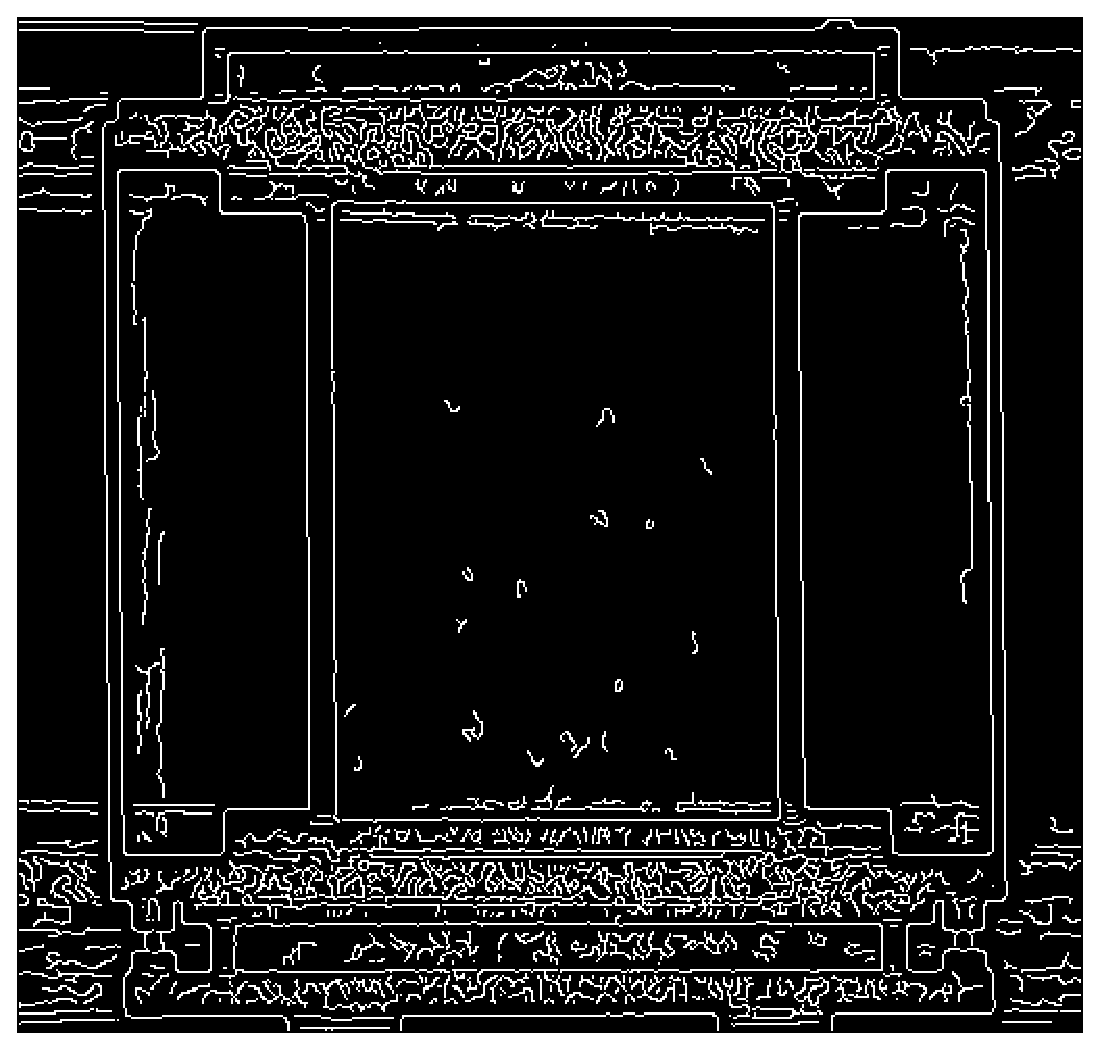
\includegraphics[width=2.75in]{data_extraction/images/canny/0.01_0.02/20121017_270.eps}}}
    \centerline{\emph{(b) Low threshold 0.01, high threshold  0.02}}
  \end{minipage}
  \begin{minipage}[t]{2.75in}
    \centering
    \centerline{\mbox{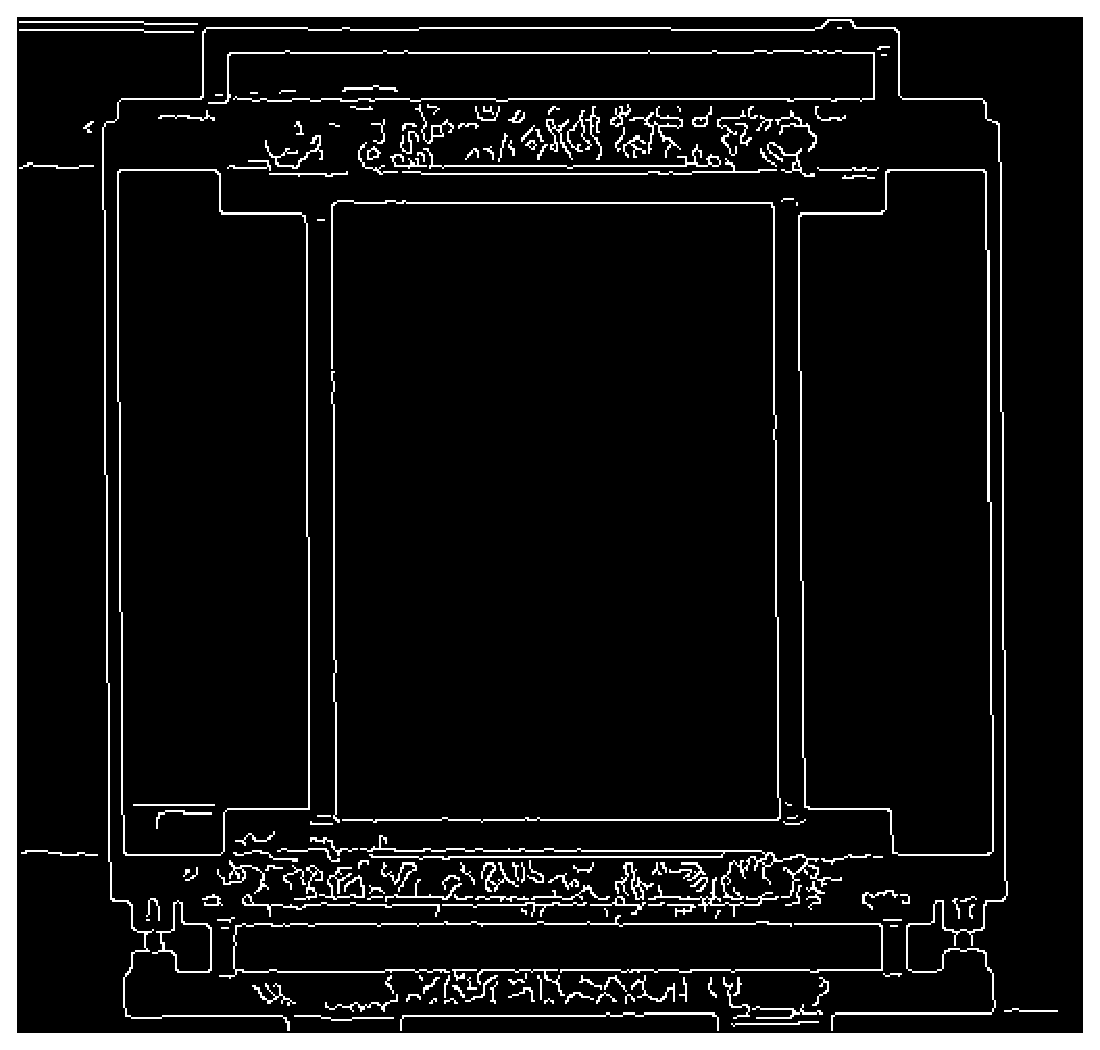
\includegraphics[width=2.75in]{data_extraction/images/canny/0.02_0.04/20121017_270.eps}}}
    \centerline{\emph{(c) Low threshold 0.02, high threshold  0.04}}
  \end{minipage}\medskip
  \begin{minipage}[t]{2.75in}
    \centering
    \centerline{\mbox{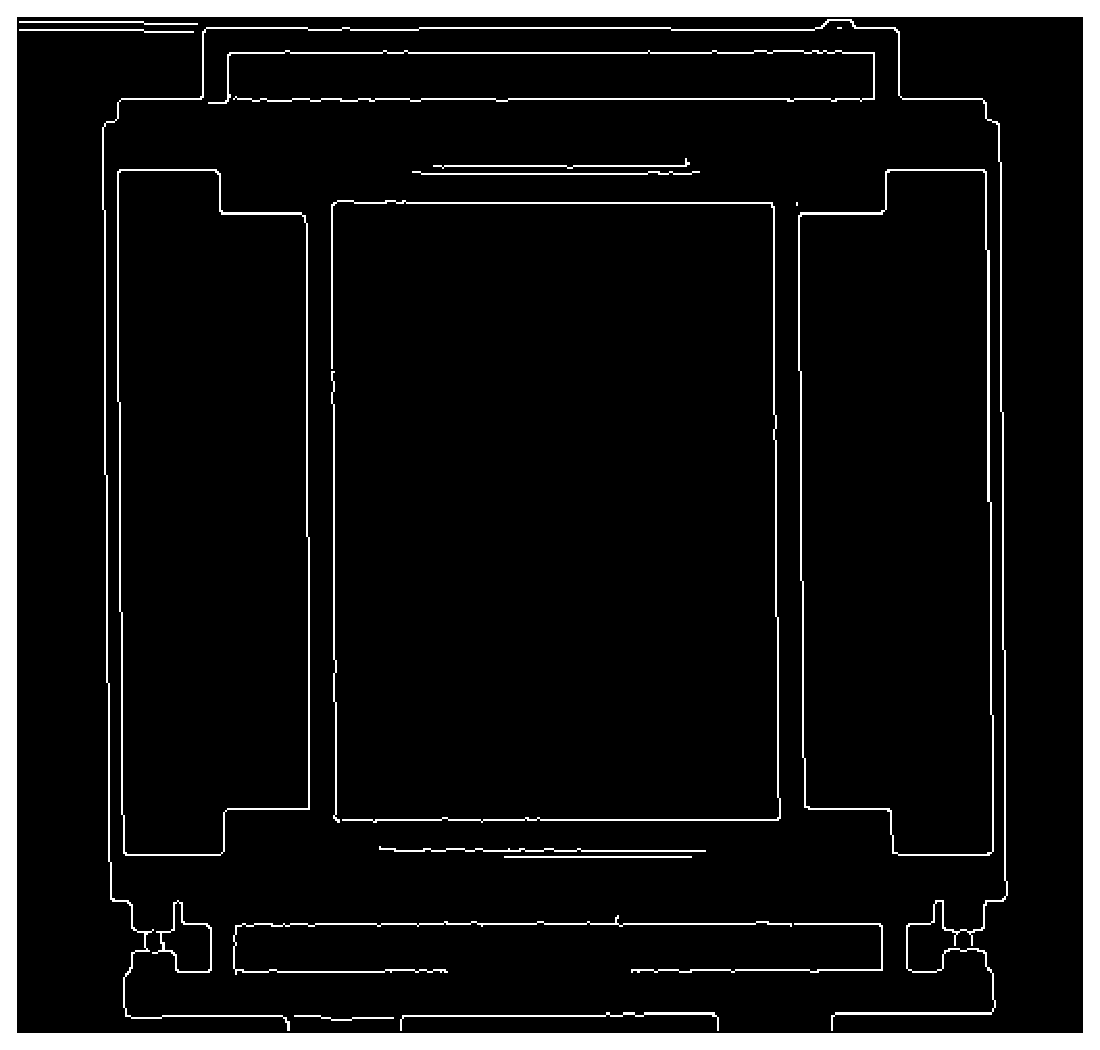
\includegraphics[width=2.75in]{data_extraction/images/canny/0.05_0.1/20121017_270.eps}}}
    \centerline{\emph{(d) Low threshold 0.05, high threshold  0.1}}
  \end{minipage}
  \caption{\emph{Canny algorithm applied to coronal sequence 270 with different parameters}} \label{fig:canny_ct_270}
\end{figure}

\begin{figure}[htb]
  \begin{minipage}[t]{2.75in}
    \centering
    \centerline{\mbox{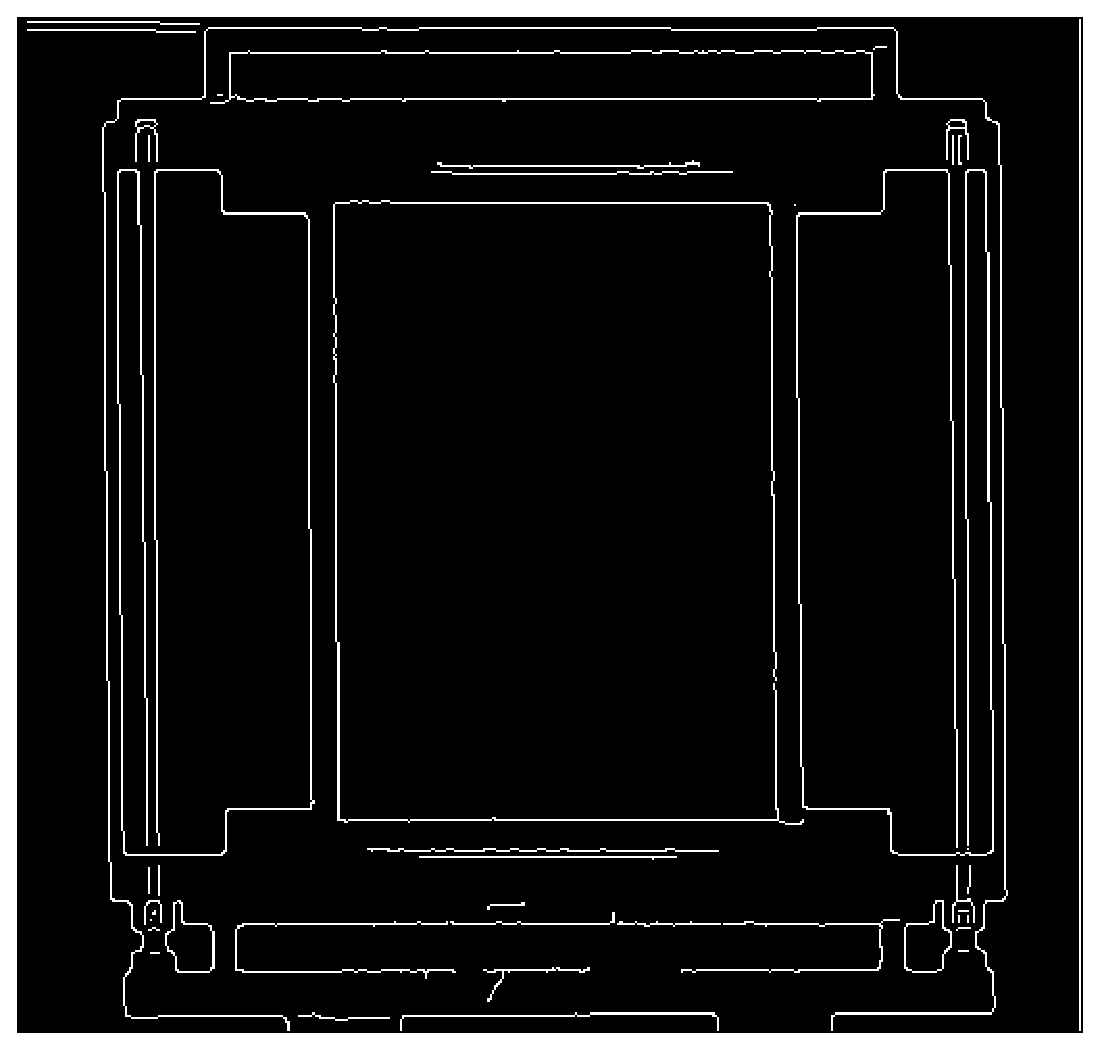
\includegraphics[width=2.75in]{data_extraction/images/canny/0.02_0.04/20121017_276.eps}}}
    \centerline{\emph{(f) Low threshold 0.02, high threshold  0.04}}
  \end{minipage}\medskip
  \begin{minipage}[t]{2.75in}
    \centering
    \centerline{\mbox{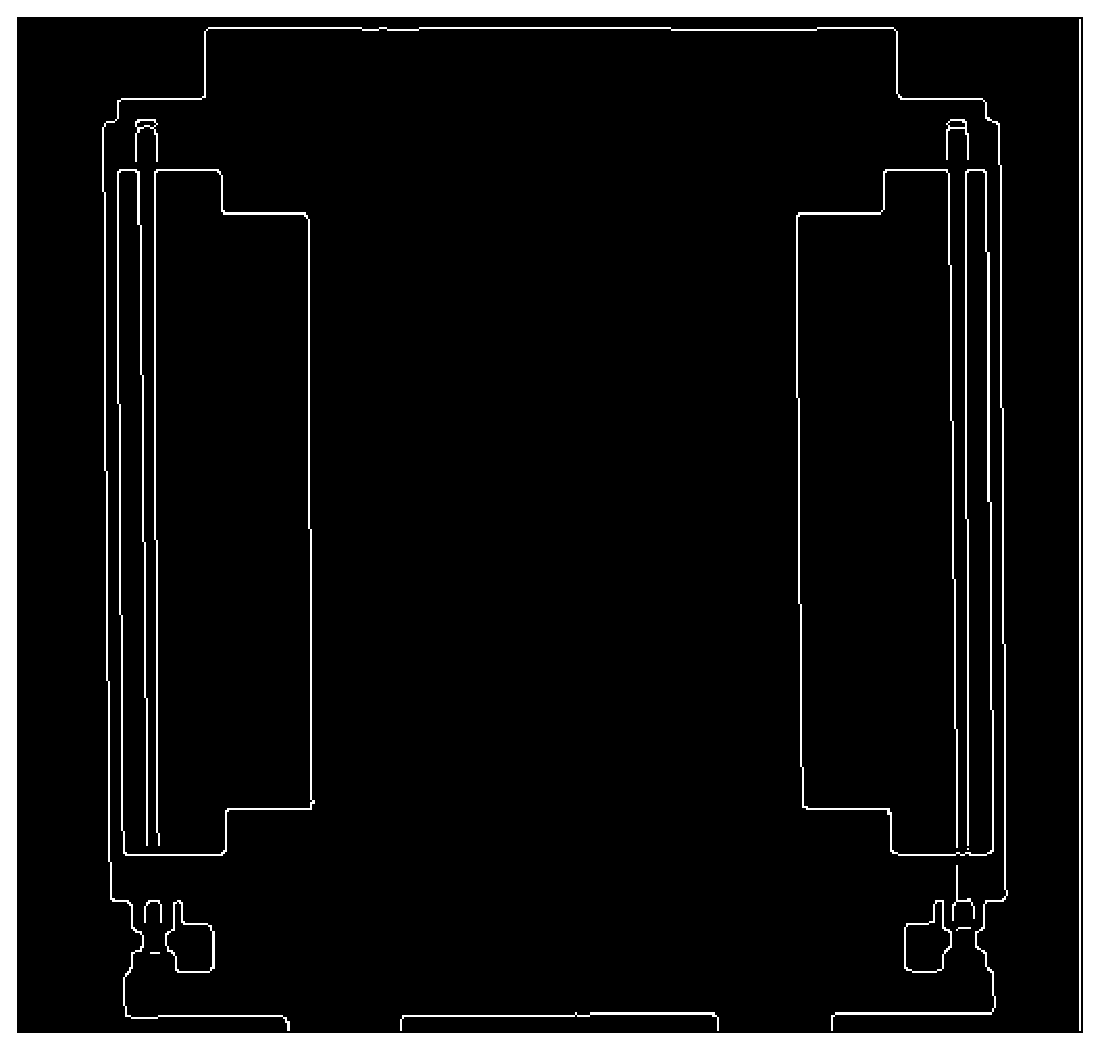
\includegraphics[width=2.75in]{data_extraction/images/canny/0.05_0.1/20121017_276.eps}}}
    \centerline{\emph{(h) Low threshold 0.05, high threshold  0.1}}
  \end{minipage}
  \caption{\emph{Canny algorithm applied to coronal sequence 276 with different parameters}} \label{fig:canny_ct_276}
\end{figure}

In figure \ref{fig:canny_ct_141}(a), we can see that Matlab's canny algorithm with default parameter gives 
descent edges when applied to image \#141. However, the same parameters will create many noisy edges in some other
images, e.g. \#270 in the same series in figure \ref{fig:canny_ct_270}(c). Setting higher threshold is able to
reduce those noisy edges as we can see in figure \ref{fig:canny_ct_270}(c), but that threshold will eliminate
some edges we are looking for as shown in \ref{fig:canny_ct_141}(c). 

To get rid of this noisy edges, different types algorithms might be involved, probably including validating
all the edges in an image,
which might involve multiple pass to the whole image, and in which case the process
could be slowed down by factor of several times. So if there is a simpler and faster way, it would be preferred
choice.

\subsection{Surface Location}

Since all objects we are looking for has a very uniform and distinct shape, we could start with finding a small 
regions each contains one object. In our case, the choice is very obvious. The objects we are looking for are
four straight lines at fixed location and parallel to each other. For images that contain those objects, they
should have them at almost exactly the same location with possibility of a few pixels offset due to potential
tiltness of the phantom during scan. If we choose a slice in the middle of the series, that should give us a
relatively smaller overall error margin both above and below the surface location on that particular slice
comparing to picking a slice at the beginning or at the end of the series which would give a relatively larger 
error on either above or below the surface location. Also the slice in the middle of series tends to have better 
quality. We would call this middle slice as surface location sample.

In the surface location sample, we would plot a histogram of gradient of the sum of middle 7 columns as shown
in figure \ref{fig:histograms_mid_coronal}(a) and a histogram of intensity distribution as shown in
figure \ref{fig:histograms_mid_coronal}(b). From figure \ref{fig:histograms_mid_coronal}(b), we can see that there
are three very obvious normal distribution in the graph. 
From left to right, they represent background noise signal, water signal and phantom tank signals respectively.
In figure \ref{fig:histograms_mid_coronal}(c), a zoomed in picture of the region between water signal distribution
and phantom tank distribution, we can see that two distributions' tails overlaps with each other. From the fact 
that the number of pixels in this overlap region is quite small and that this region is between two 
distributions, we can determine that most of them should be the pixels on the boundary between water and tank.
So, according to ranges of two distributinos as we can observer from the diagram, the range of difference
between tank signal and water signal should be somewhere between 40 to 300. However, since the difference we are
looking for is on the boundary of water and phantom tank, signals in those regions should tend to be close 
to each other. Therefore we should expect the to see spikes in gradient to be around $\pm40$. In figure
\ref{fig:histograms_mid_coronal}(a), we can clearly see six spikes that can be uniquely identified.
Their values are -41.8404, 44.2372, -36.2271, 50.4055, -40.9654 and 29.8124, and they are right around the 
predicted range. Thus, we can identify them with high confidence that they are on each of the boundary between
water and phantom tank.

With one pixel on each locations of the water and phantom tank boundaries are identified, 
we can also narrow down the 
location of each surface by specifying the surfaces are within the $\pm5$ rows of the row coordinate of each
identified pixels. The $\pm5$ rows should give enough room for any horizontal or vertical tiltness.

\begin{figure}[htb]
  \begin{minipage}[t]{2.75in}
    \centering
    \centerline{\mbox{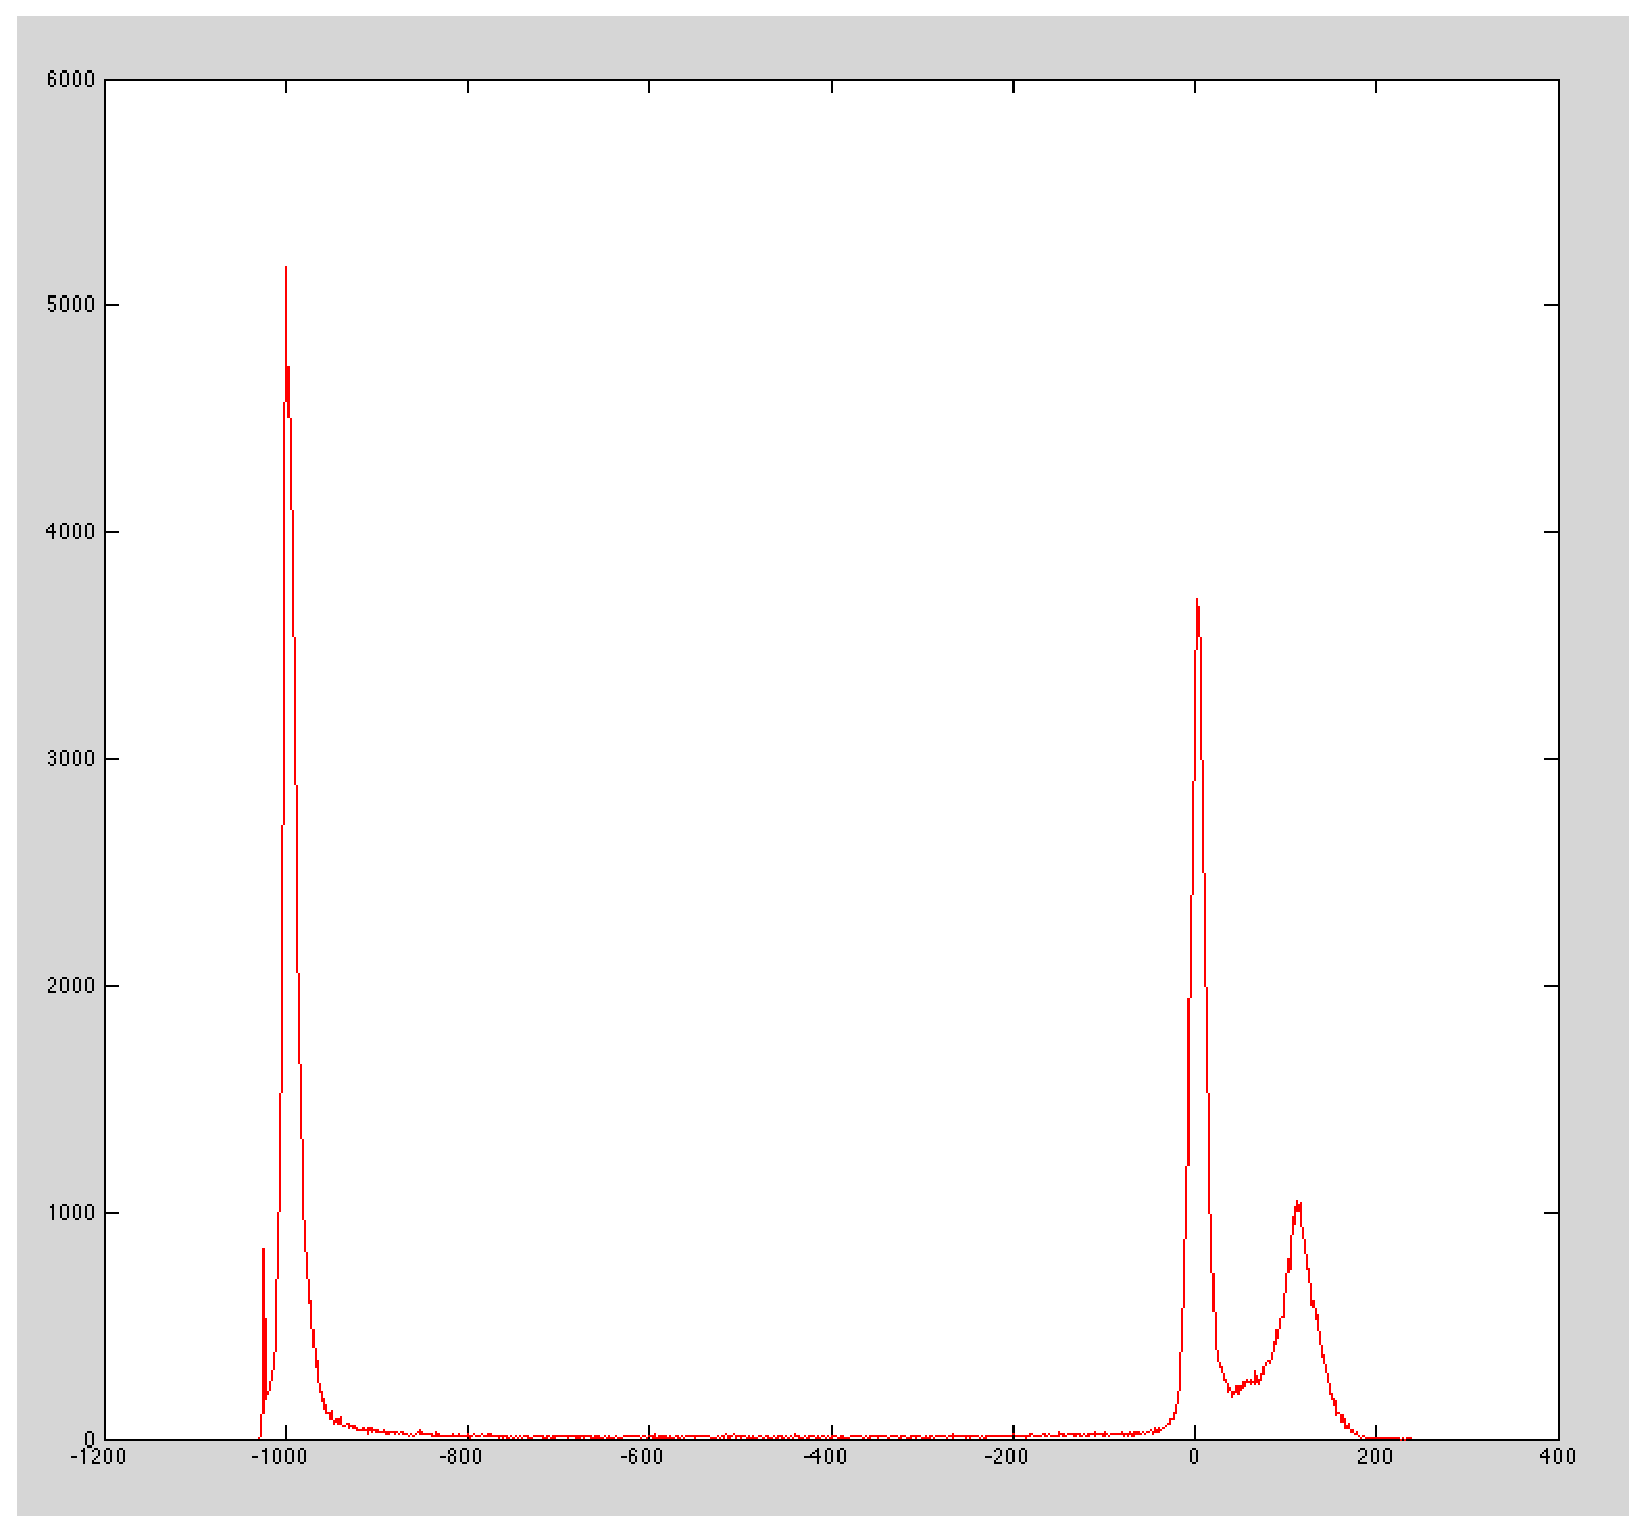
\includegraphics[width=2.75in]{data_extraction/images/mid_slice_histogram.eps}}}
    \centerline{\emph{(a) mid slice intensity histogram}}
  \end{minipage}\medskip
  \begin{minipage}[t]{2.75in}
    \centering
    \centerline{\mbox{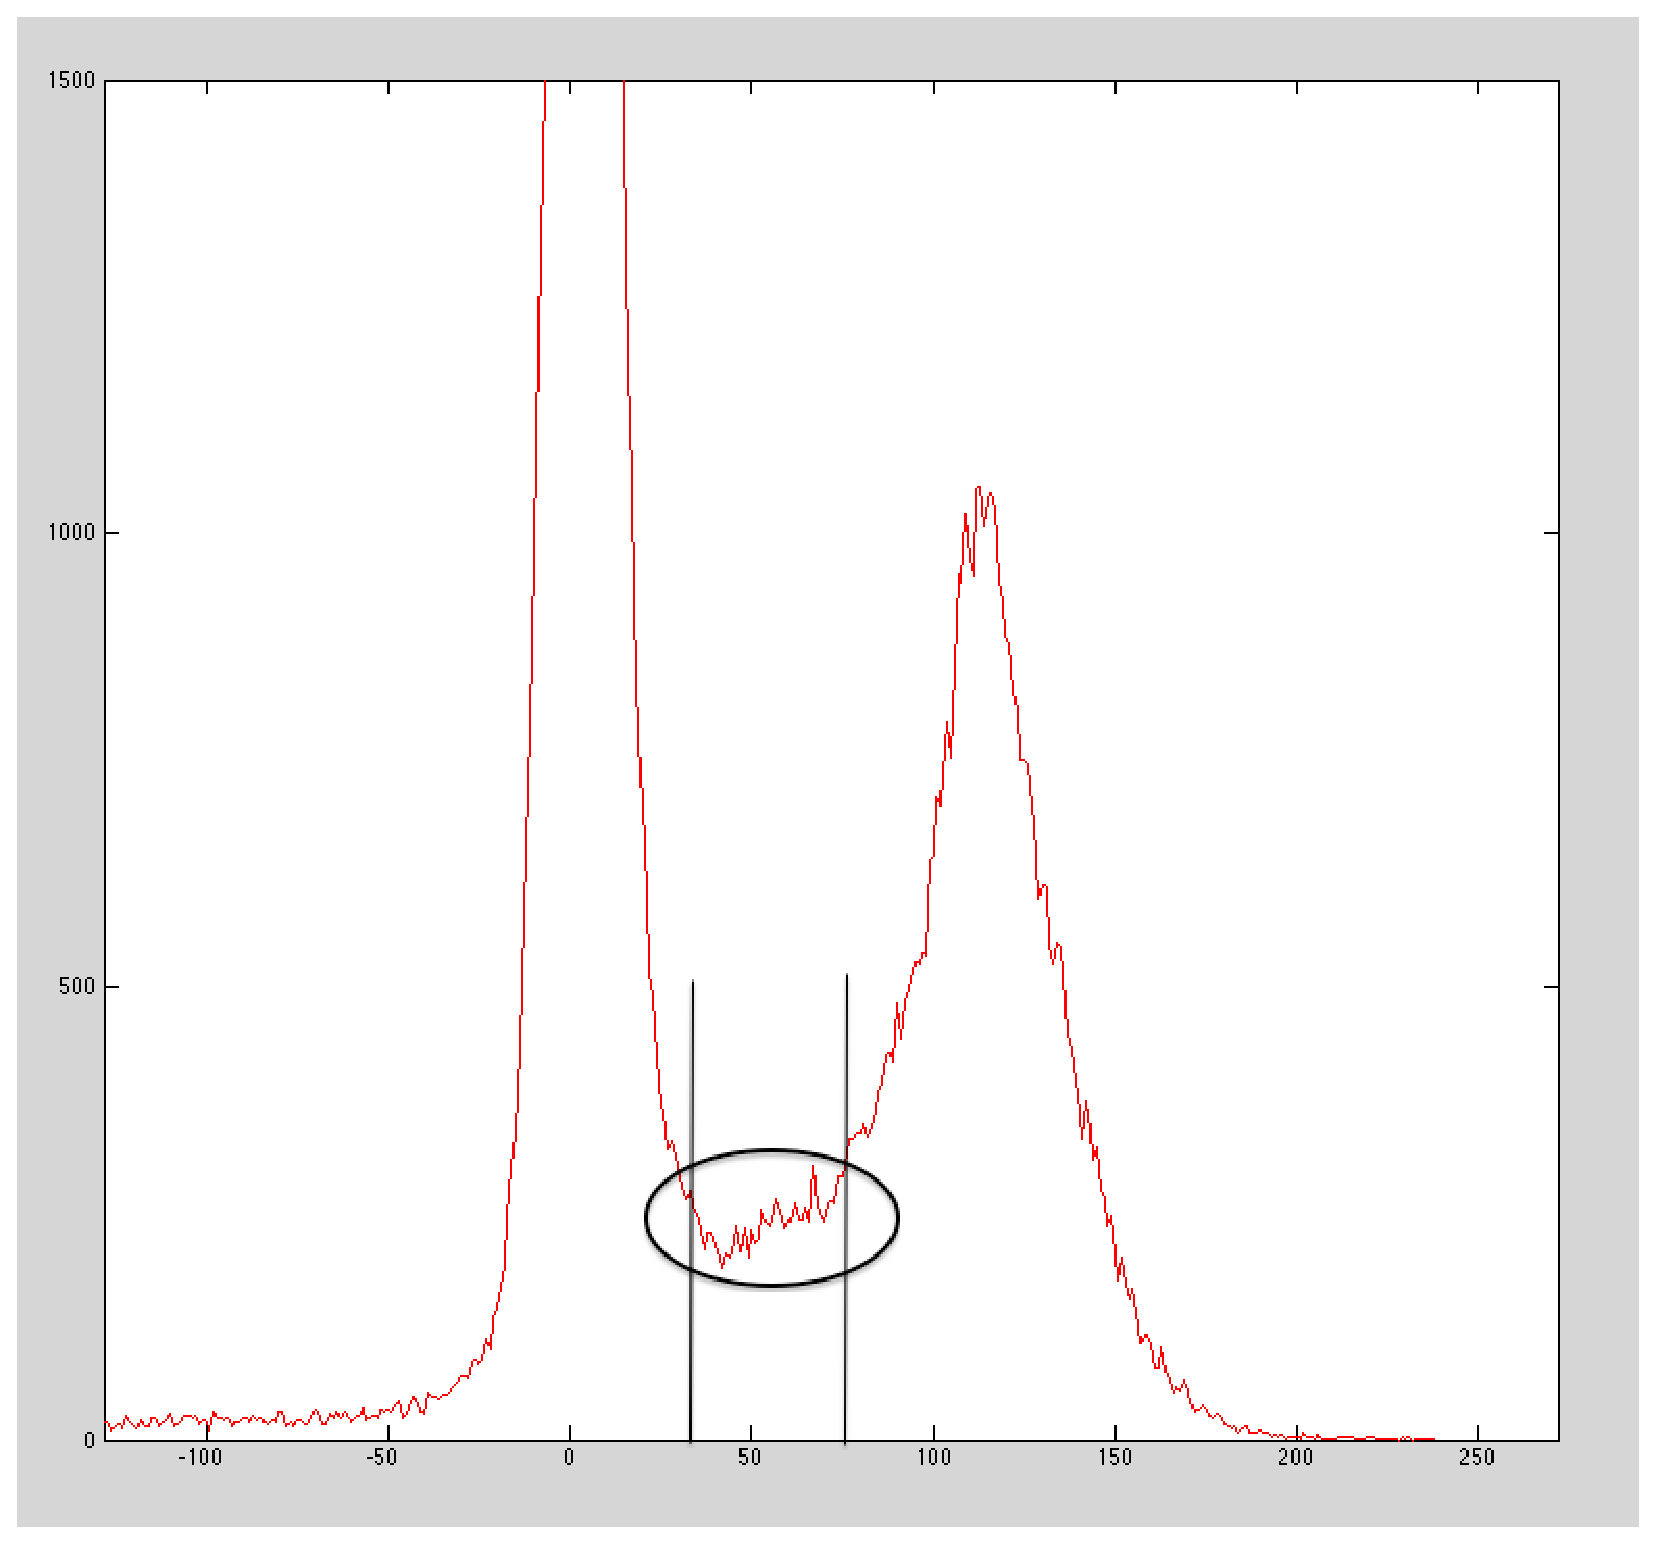
\includegraphics[width=2.75in]{data_extraction/images/mid_slice_tank_and_water_overlap_marked.eps}}}
    \centerline{\emph{(b) Mared overlap region}}
  \end{minipage}
  \begin{minipage}[t]{2.75in}
    \centering
    \centerline{\mbox{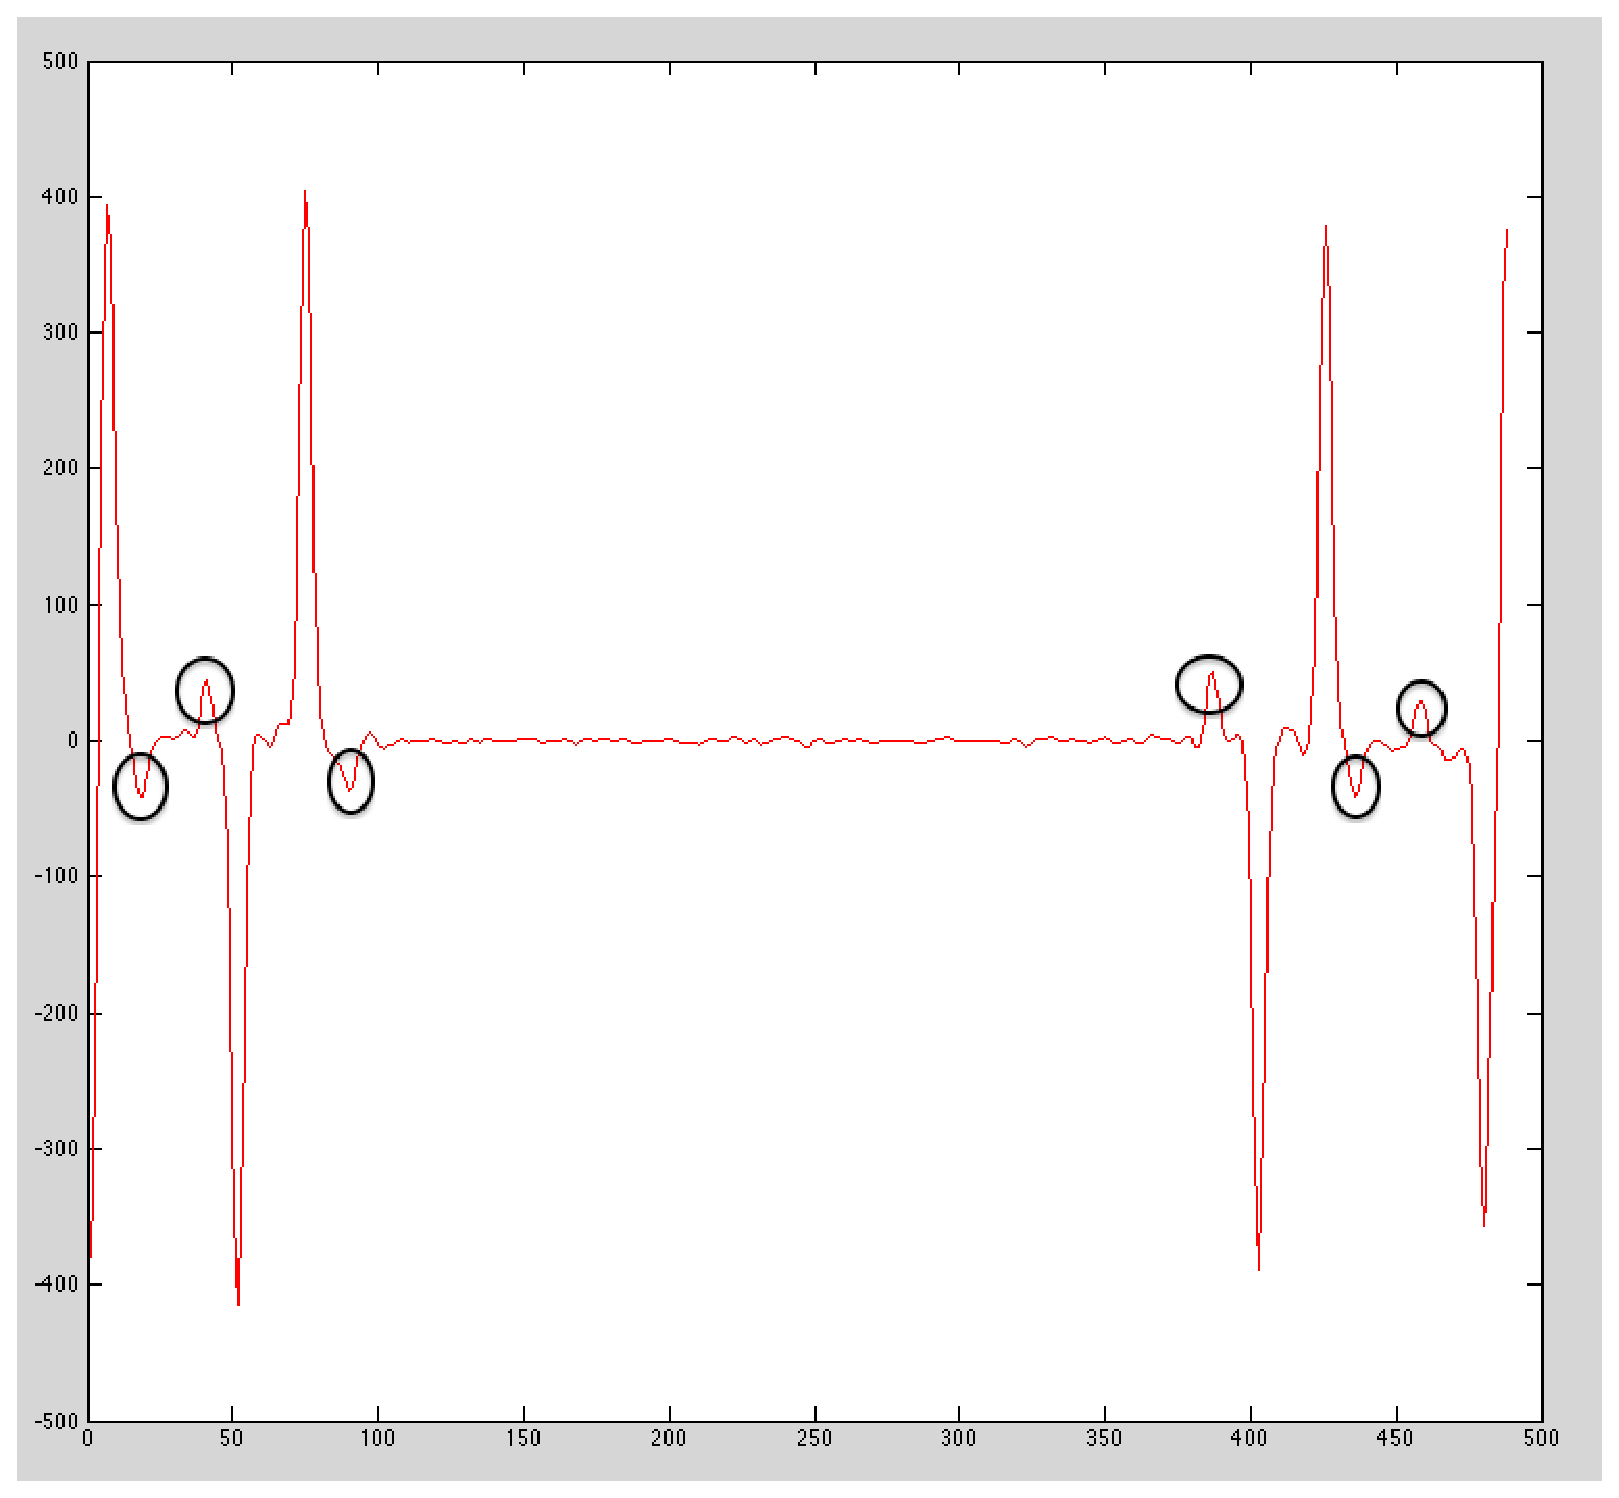
\includegraphics[width=2.75in]{data_extraction/images/mid_slice_gradient_marked.eps}}}
    \centerline{\emph{(c) mid slice surface locations}}
  \end{minipage}

  \caption{\emph{Histograms of middle column of middle slice of a coronal series}} 
  \label{fig:histograms_mid_coronal}
\end{figure}

\subsection{Edge Detection On Local Surface Region}

After the regions of boundaries of water and phantom tank are extract we can proceed to extract the surface
edge from these regions. The following issues are need to be resolved:
\begin{enumerate}
  \item Identify the left and right boundaries of the edges.
  \item Remove the noisy edges, and there are two types noisy edges:
    \begin{enumerate}
      \item Noisy edges that are not in contact with the target edge.
      \item Noisy edges that are in contact with the target edge.
    \end{enumerate}
\end{enumerate}

\subsubsection{Boundary Finding}

To detect the left and right boundary we plot the histogram of sum of intensities of each column across the
region as well as the gradient for the intensity graph as shown in figure 
\ref{fig:coronal_270_boundary_histogram}. 

\begin{figure}[htb]
  \begin{minipage}[t]{5in}
    \centering
    \centerline{\mbox{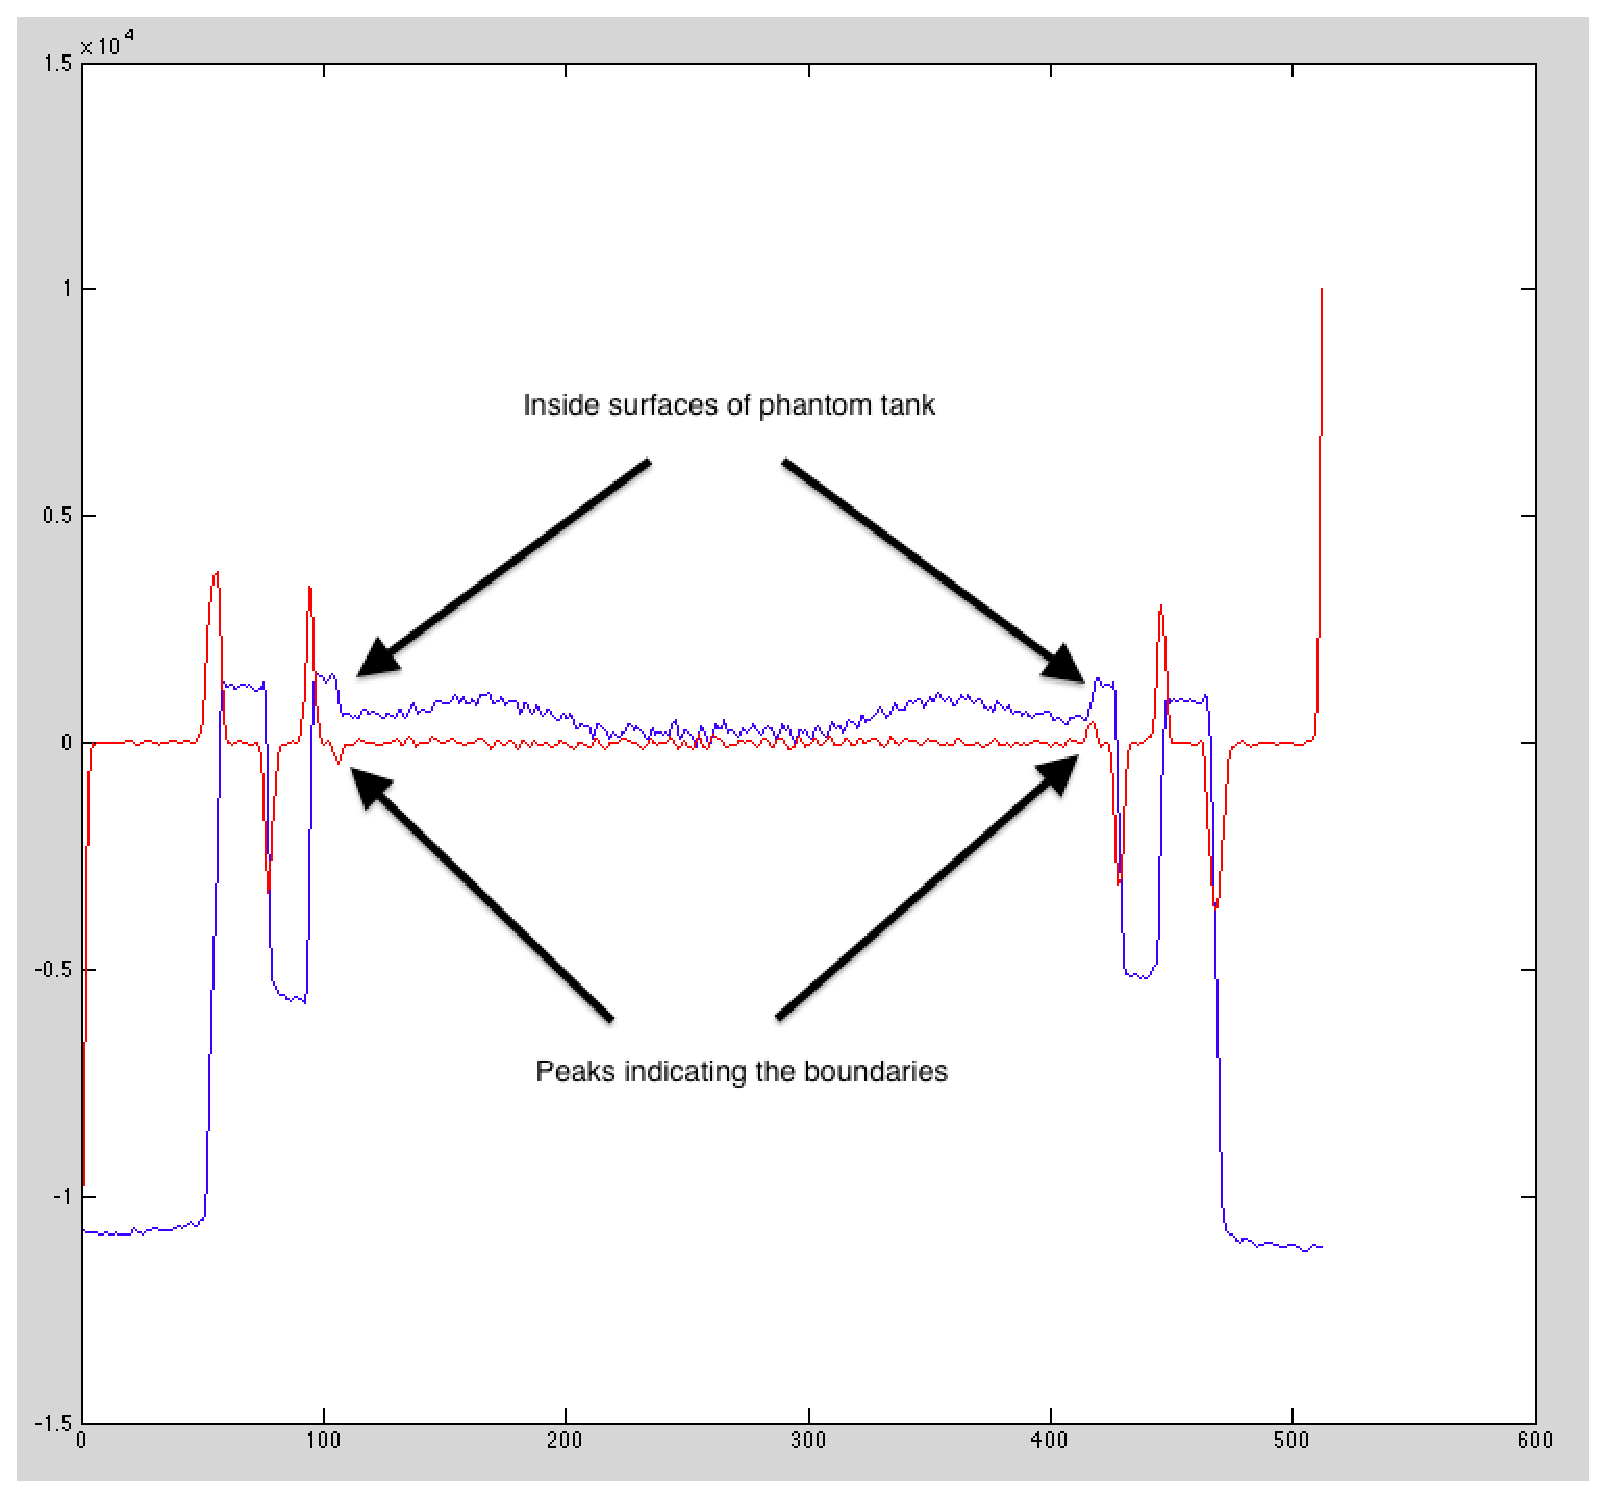
\includegraphics[width=5in]{data_extraction/images/sample/20121017_270/Coronal/inferior_inside/histogram_marked.eps}}}
    \centerline{\emph{(a) Histogram for inferior tank inside edge}}
  \end{minipage}
  \caption{\emph{Histogram for boundary detection on image sequence \#270}}
  \label{fig:coronal_270_boundary_histogram}
\end{figure}

\begin{figure}[htb]
  \begin{minipage}[t]{5in}
    \centering
    \centerline{\mbox{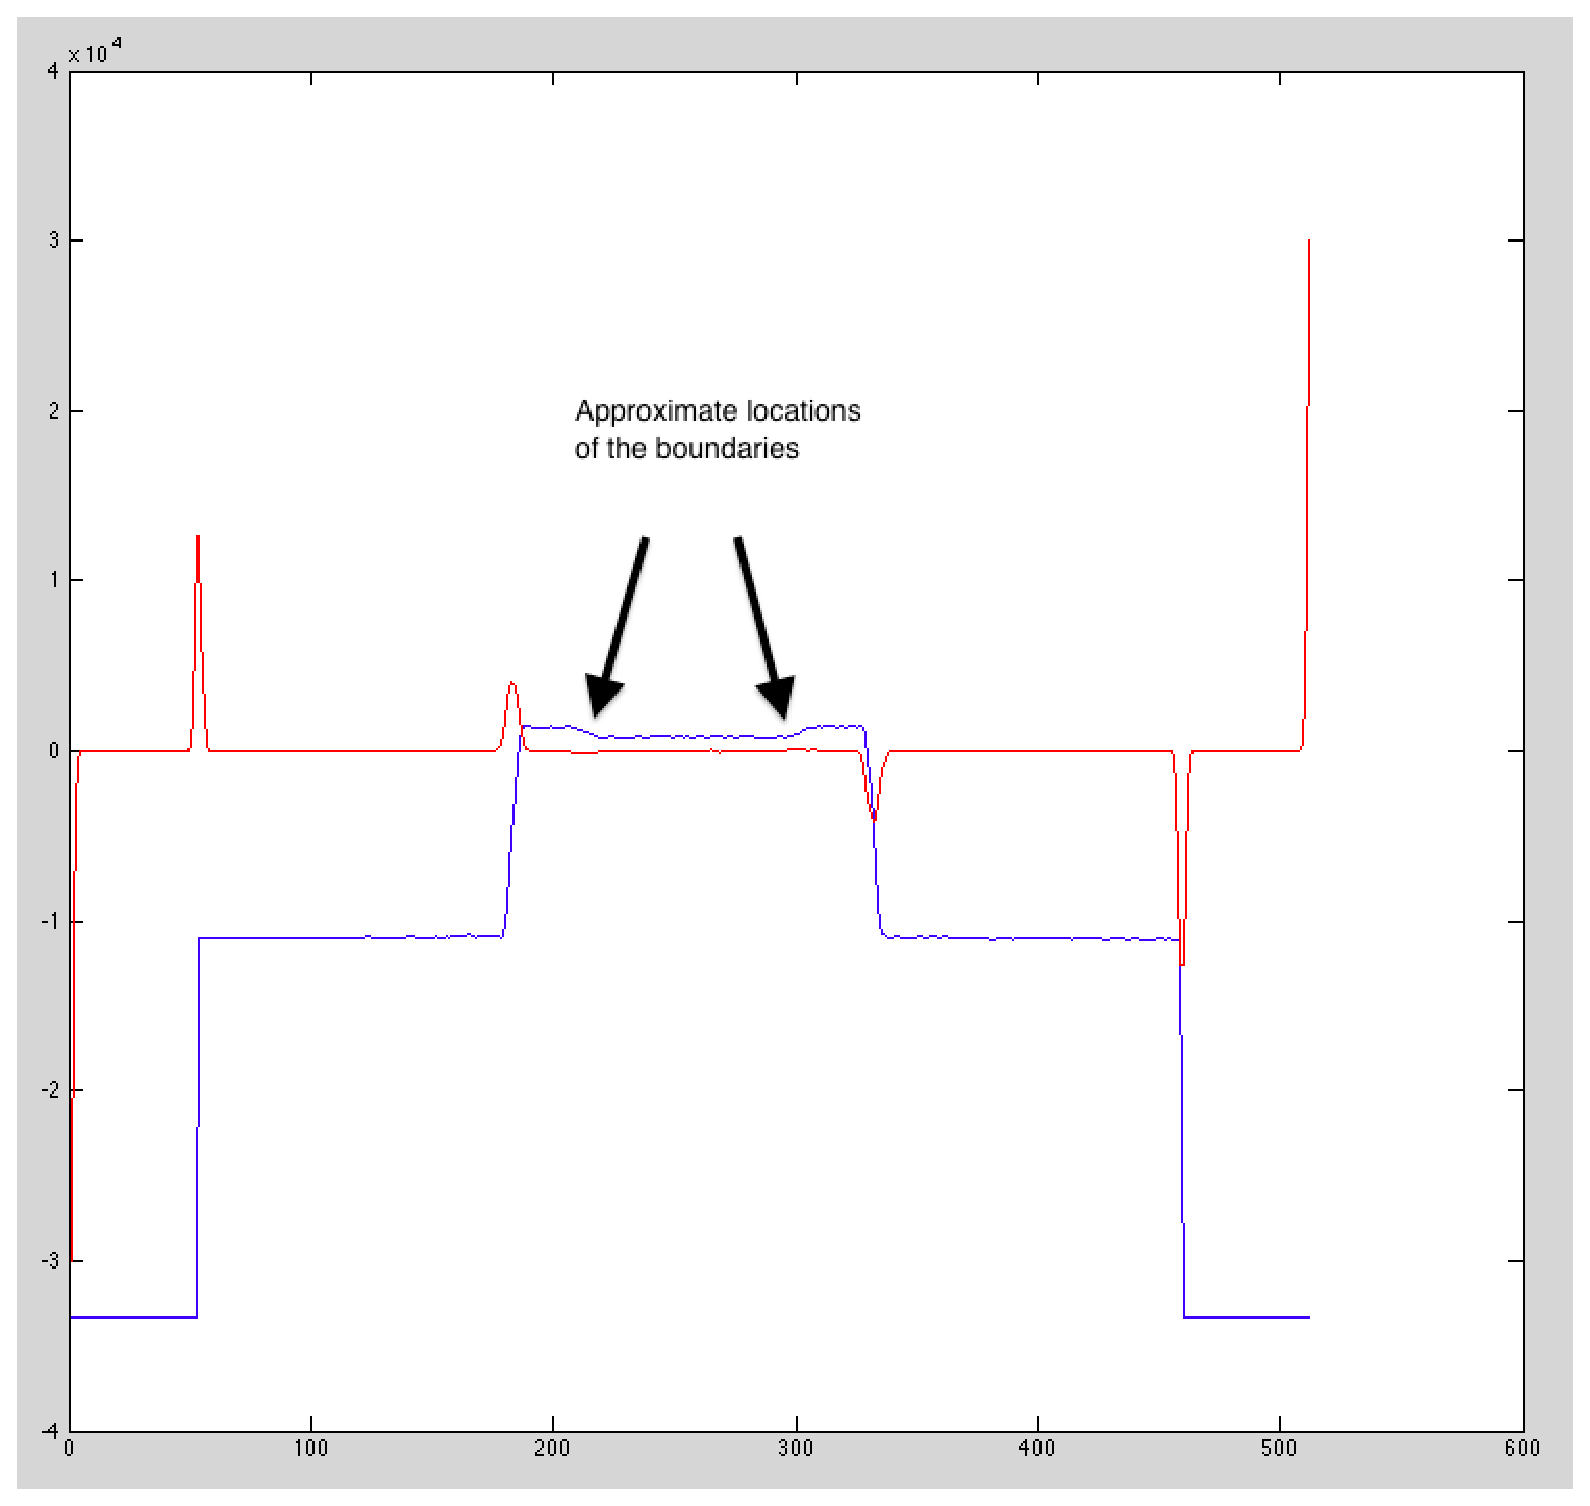
\includegraphics[width=5in]{data_extraction/images/sample/20121017_100/Coronal/superior_outside/superior_outside_histogram_marked.eps}}}
    \centerline{\emph{(a) Histogram for superior tank outside edge}}
  \end{minipage}
  \caption{\emph{Histogram for boundary detection on image sequence \#100}}
  \label{fig:coronal_270_boundary_histogram}
\end{figure}

Upper pair of arrows in figure \ref{fig:coronal_270_boundary_histogram} indicates where the inside edges of
the phantom tanks are, and the lower pair of arrows indicates how do those edges shows up in its gradient graph.
The two small edges are identifiable with properties of value bewteen 200 and 1000. We can identify them with
this property for most of the sliceds. The transition from phantom tank to water become smoother on the slices
more toward anterior or posterior in coronal view. 

There are couple of issues with this approach.
\begin{itemize}
  \item For images close to either edges of the two tanks, contrast ratio between water and tank material 
    become very weak. As shown in figure \ref{fig:coronal_edge_final_result}, the transition from tank to
    water become very smooth, and their gradient, therefore, become very small, and fallen out the filter
    range we specified. If we lower the range of the filter, it will pick up too many noise.
  \item For superior tank's outside surface, its regions also include the end part of tubes. Structure
    on those regions of tubes are fairly complex, which will result in frequent change of each column's 
    total intensities in regions that have tubes.
% so there are lots of change of peaks in the intensity 
%     graph as we can see in figure \ref{fig:superior_outside_artifacts}, and it's easy for some of these peaks to fall into the range of our
%     boundary filter. 
\end{itemize}

\begin{figure}[htb]
  \begin{minipage}[t]{2.75in}
    \centering
    \centerline{\mbox{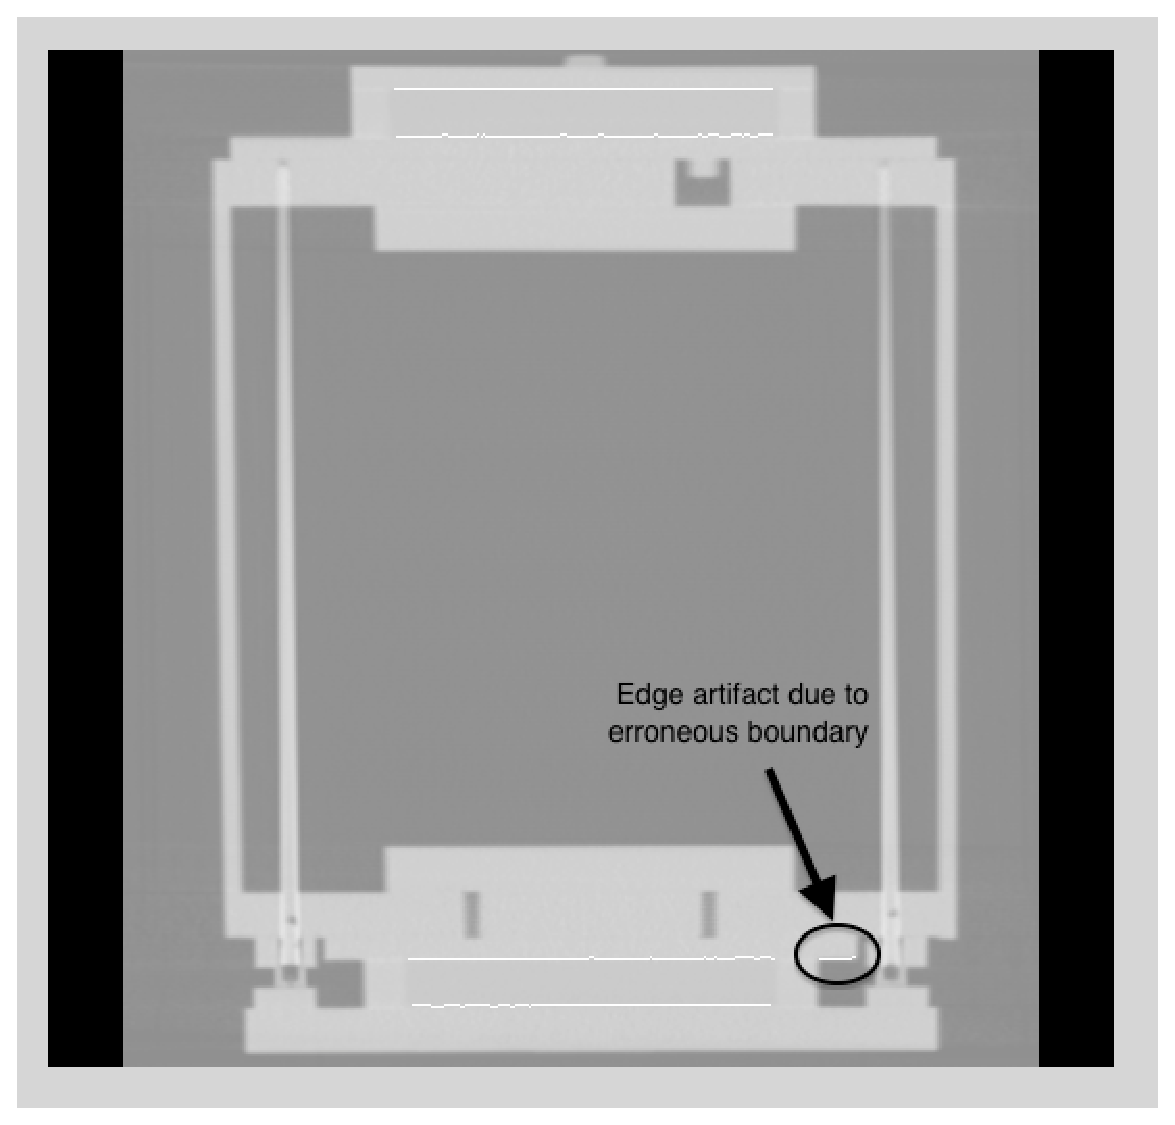
\includegraphics[width=2.75in]{data_extraction/images/sample/20121017_125/Coronal/Superior_outside/extra_edge.eps}}}
    \centerline{\emph{(a) Extra edge caused by tube section}}
  \end{minipage}
  \begin{minipage}[t]{2.75in}
    \centering
    \centerline{\mbox{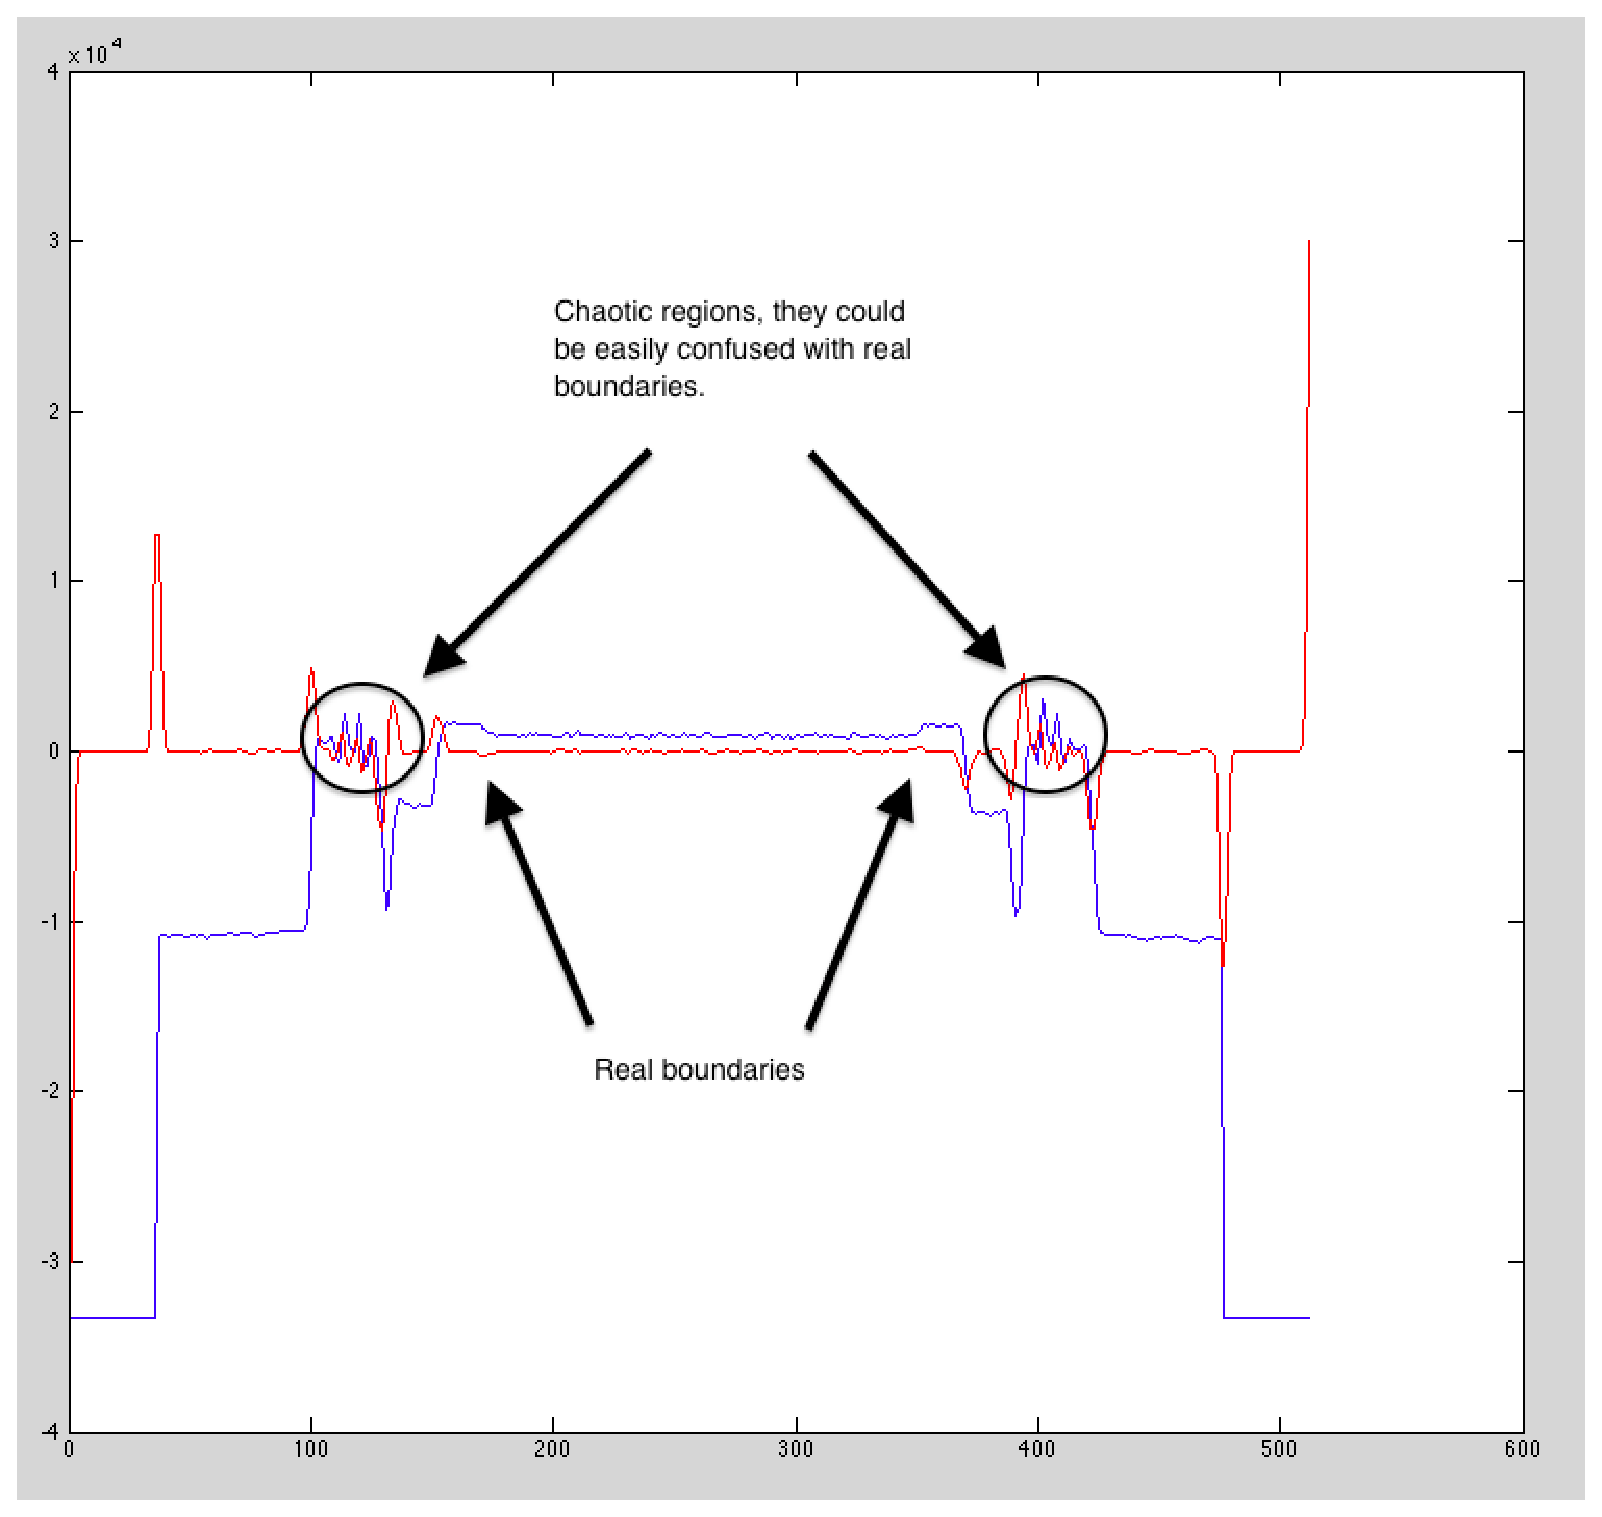
\includegraphics[width=2.75in]{data_extraction/images/sample/20121017_125/Coronal/Superior_outside/extra_edge_histogram.eps}}}
    \centerline{\emph{(b) Histgram of the superior outside surface in (a) }}
  \end{minipage}
  \caption{\emph{Superior outside surface artifacts}}
  \label{fig:superior_outside_artifacts}
\end{figure}

However, with the slices that able to identify the edges,
we can reconstruct majority of each water tank surface and they are more than enough for us to estimate the
distances between each surfaces, especially with the assumption that they are all flat and parallel to each
other.

\subsubsection{Removing Noise}

We are going to remove the noise of the each edge in two steps. 
\begin{enumerate}
  \item Remove noisy edges that are unattached to target edges.
  \item Filter out small edges sticking out of target edges. 
\end{enumerate}

Noisy edges unattached to target edges has one characteristic which is short. Since these edges are generated
by noises, all observations has shown that they all tend to be very short in length due to lack of consistent
pattern. To remove the noisy edges that are unattached to the target edges, we do the following steps:
\begin{enumerate}
  \item Create an empty image that has the same size of the input image.
  \item Iterate every pixel of input image
    \begin{enumerate}
      \item if current pixel in input image is not zero:
        \begin{enumerate}
          \item We recursively collect all the nonzero pixels from the input image and set those pixel values on
            the input image to 0.
        \end{enumerate}
      \item If there has been an edge collected, we check the length of this group of pixels
        \begin{enumerate}
          \item If the length is less than a threshold, say, 15, we assume they are a noisy edge and 
            complete ignore this group of pixels
          \item Otherwise, we will write these pixels' values to the image we initially created.
        \end{enumerate}
    \end{enumerate}
\end{enumerate}

After follwing above steps, the resulting image will look like something like figure 
\ref{fig:coronal_270_intermediate_results} (c).

At this stage, we will apply the boundary limit to this newly filtered edge, removing all the pixels beyond
either left or right boundary. And this will left us with target edges with some small noisy edges sticking
out as shown in figure \ref{fig:coronal_270_intermediate_results} (d).

To filter these sticking edges out, we do the following steps:

\begin{enumerate}
  \item Extract 2d coordinate informate of every edge pixels, and fit them to a straight line, since we know
    our target edge is a straight line. We can setup the equation as:
    \begin{eqnarray}
      \begin{bmatrix}
        columns \quad 1
      \end{bmatrix}
      \begin{bmatrix}
        m\\
        k\\
      \end{bmatrix}
      & = & 
      \begin{bmatrix}
        rows
      \end{bmatrix}
    \end{eqnarray}
    where \emph{columns} is column values of all edge pixels and \emph{rows} is row values of all edge pixels.
    $m$ and $k$ will the line parameter of the straight line we are trying to fit into.
  \item Group all edge pixels by their column value.
  \item Iterate all column groups. We pick a pixel from each group having the minimum value of
    $|Pixel_{row} - (m*Pixel_{column} + k)|$ and ignore the rest.
  \item At the end we should have one pixel per column group left, they will be our final edge.
\end{enumerate}

For testing we write out these filtered edges to original input image. We can see the result in figure 
\ref{fig:coronal_edge_final_result} (a). For some edges, in some image we are unable to determine the left
and right boundary. We will skip them as we have more than enough data with images that can gives us good 
edges. Figure Figure \ref{fig:coronal_edge_final_result} (b) is an example where some edges are identifiable
while others not.

\begin{figure}[htb]
  \begin{minipage}[t]{2.75in}
    \centering
    \centerline{\mbox{
\includegraphics[width=2.75in]{data_extraction/images/sample/20121017_270/Coronal/inferior_inside/1_region.eps}}}
    \centerline{\emph{(a) Extracted region}}
  \end{minipage}\medskip
  \begin{minipage}[t]{2.75in}
    \centerline{\mbox{
\includegraphics[width=2.75in]{data_extraction/images/sample/20121017_270/Coronal/inferior_inside/2_raw_edges.eps}}}
    \centerline{\emph{(b) Raw edges}}
  \end{minipage}
  \begin{minipage}[t]{2.75in}
    \centerline{\mbox{
\includegraphics[width=2.75in]{data_extraction/images/sample/20121017_270/Coronal/inferior_inside/3_removed_noise.eps}}}
    \centerline{\emph{(c) Removed noisy edges}}
  \end{minipage}\medskip
  \begin{minipage}[t]{2.75in}
    \centerline{\mbox{
\includegraphics[width=2.75in]{data_extraction/images/sample/20121017_270/Coronal/inferior_inside/4_within_boundary.eps}}}
    \centerline{\emph{(d) Edges within the boundary}}
  \end{minipage}
  \caption{\emph{Edge extraction intermediate results on image sequence \#270's inferior tank inside edge}}
  \label{fig:coronal_270_intermediate_results}
\end{figure}

\subsubsection{Improvement}



\begin{figure}[htb]
  \begin{minipage}[t]{2.75in}
    \centering
    \centerline{\mbox{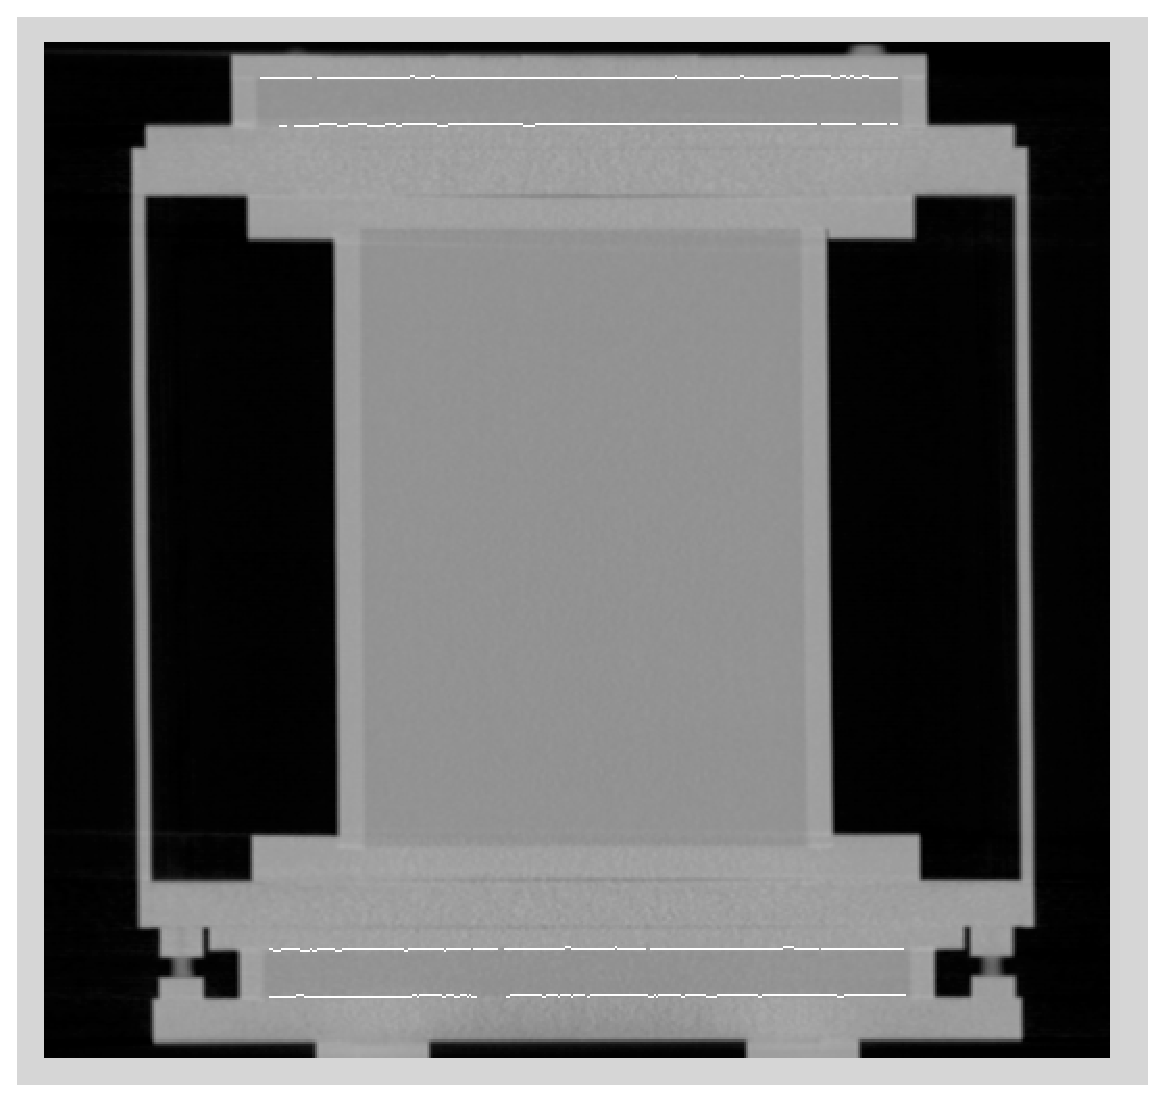
\includegraphics[width=2.75in]{data_extraction/images/sample/20121017_270/Coronal/result.eps}}}
    \centerline{\emph{(a) Edge result on image sequence \#270}}
  \end{minipage}
  \begin{minipage}[t]{2.75in}
    \centering
    \centerline{\mbox{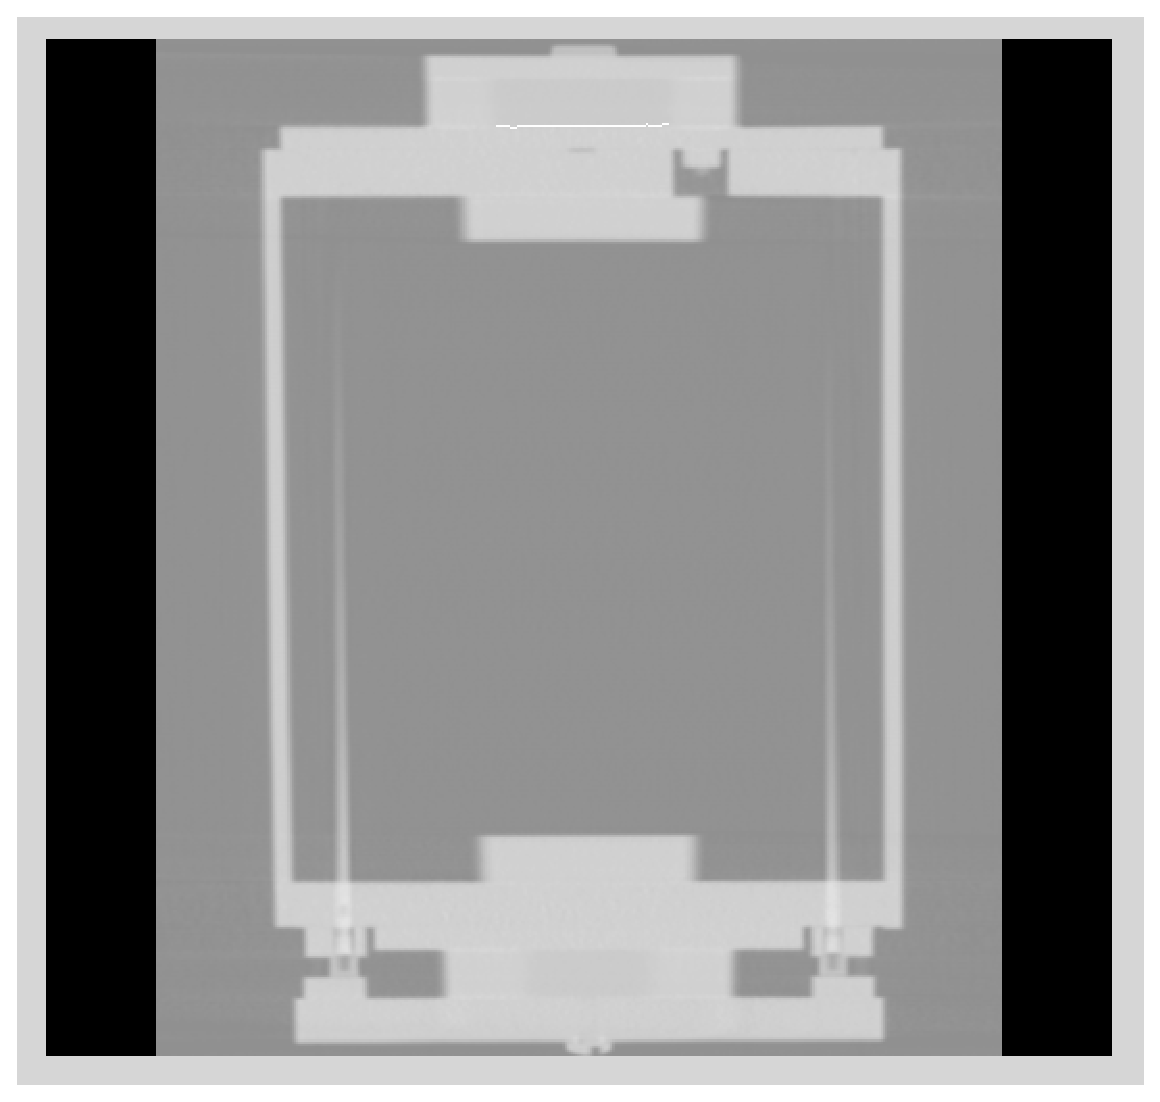
\includegraphics[width=2.75in]{data_extraction/images/sample/20121017_100/Coronal/result_canny_[0.001,0.002].eps}}}
    \centerline{\emph{(b) Edge result on image sequence \#100}}
  \end{minipage}
  \caption{\emph{Final edge results}}
  \label{fig:coronal_edge_final_result}
\end{figure}


\subsection{Creating Surfaces}

Surface in 3D space can be represented by equation:
\begin{eqnarray}
ax + by + cz + d & = & 0 \label{eq:plane}
\end{eqnarray}

With somewhere between 50,000~70,000 date points for each surfaces, it's the best to use least square ($Ax=b$) to 
esitmate each surfaces' equation paramters. Considering the following fact:
\begin{enumerate}
  \item Least square assumes that there is error in measurement but not observation, so it will only try to
    minimize error in A not b.
  \item For every data point we only have measurement error in two axis, the third one is taking for granted 
    from DICOM info. Though there should be some very small error during CT image reconstruction as well, but
    that's not necessary to be consider here.
\end{enumerate}
Since the image set we are dealing with is coronal view, which means it's the y-axis we are taking for granted,
we are setting up our least square as follows:

\begin{eqnarray}
\frac{a}{b}x + \frac{c}{b}z + \frac{d}{b} & = & -y \label{eq:x_orient}\\
\begin{bmatrix}
  x_0  & z_0 & 1 \\
  \vdots & \vdots & \vdots \\
  x_n & z_n & 1 \\
\end{bmatrix}
\begin{bmatrix}
a/b\\
c/b\\
d/b
\end{bmatrix}
& = &
\begin{bmatrix}
-y_0 \\
\vdots\\
-y_n
\end{bmatrix}
\end{eqnarray}

With this setup, our estimated paramters for each planes are:

\begin{tabular}{| l || r | r | r | r |}
            \hline
            &               $a$ & $b$ &               $c$ & $d$ \\
            \hline
  surface 1 & $-1.0617\times10^{-06}$ & $1$ & $-6.9880\times10^{-10}$ & $-2.0644$ \\ 
            \hline
  surface 2 & $-3.8209\times10^{-06}$ & $1$ & $-2.3851\times10^{-9}$  & $-6.7681$ \\ 
            \hline
  surface 3 & $3.2496\times10^{-06}$  & $1$ & $4.3242\times10^{-10}$  & $-4.8297$ \\ 
            \hline
  surface 4 & $3.3399\times10^{-06}$  & $1$ & $1.2575\times10^{-10}$  & $-2.0644$ \\ 
            \hline
\end{tabular}

% algorithm limited by two factors:
% \begin{enumerate}
%   \item left and right boundary finding
%   \item canny parameters
% \end{enumerate}

% continue here $\dots$

Reconstructed surfaces can be see below:

\begin{figure}[htb]
  \begin{minipage}[t]{2.75in}
    \centering
    \centerline{\mbox{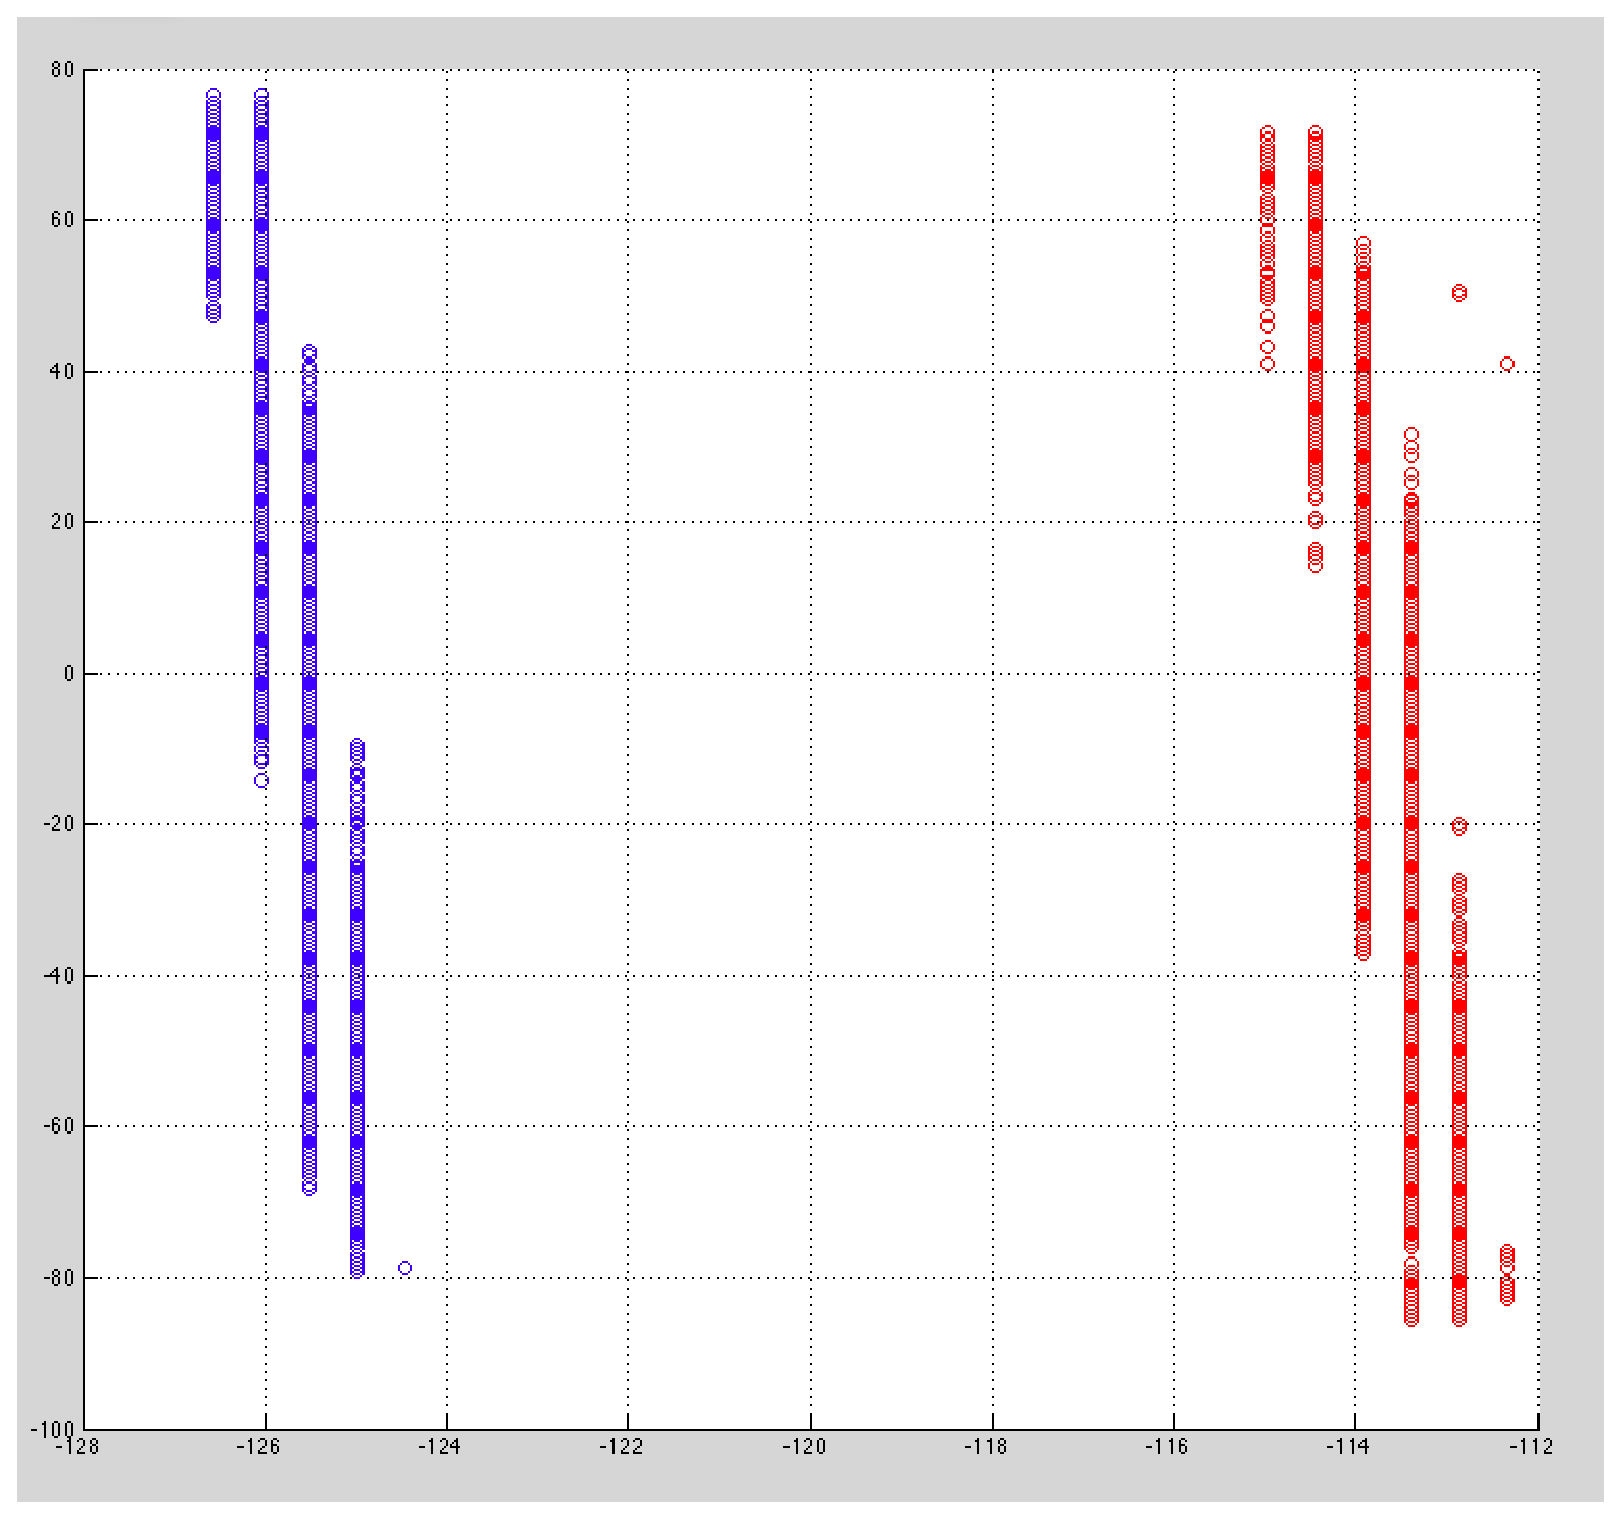
\includegraphics[width=2.75in]{data_extraction/images/surface_plane/superior_comparison/Surface1_2.eps}}}
    \centerline{\emph{(a)}}
  \end{minipage}\medskip
  \begin{minipage}[t]{2.75in}
    \centering
    \centerline{\mbox{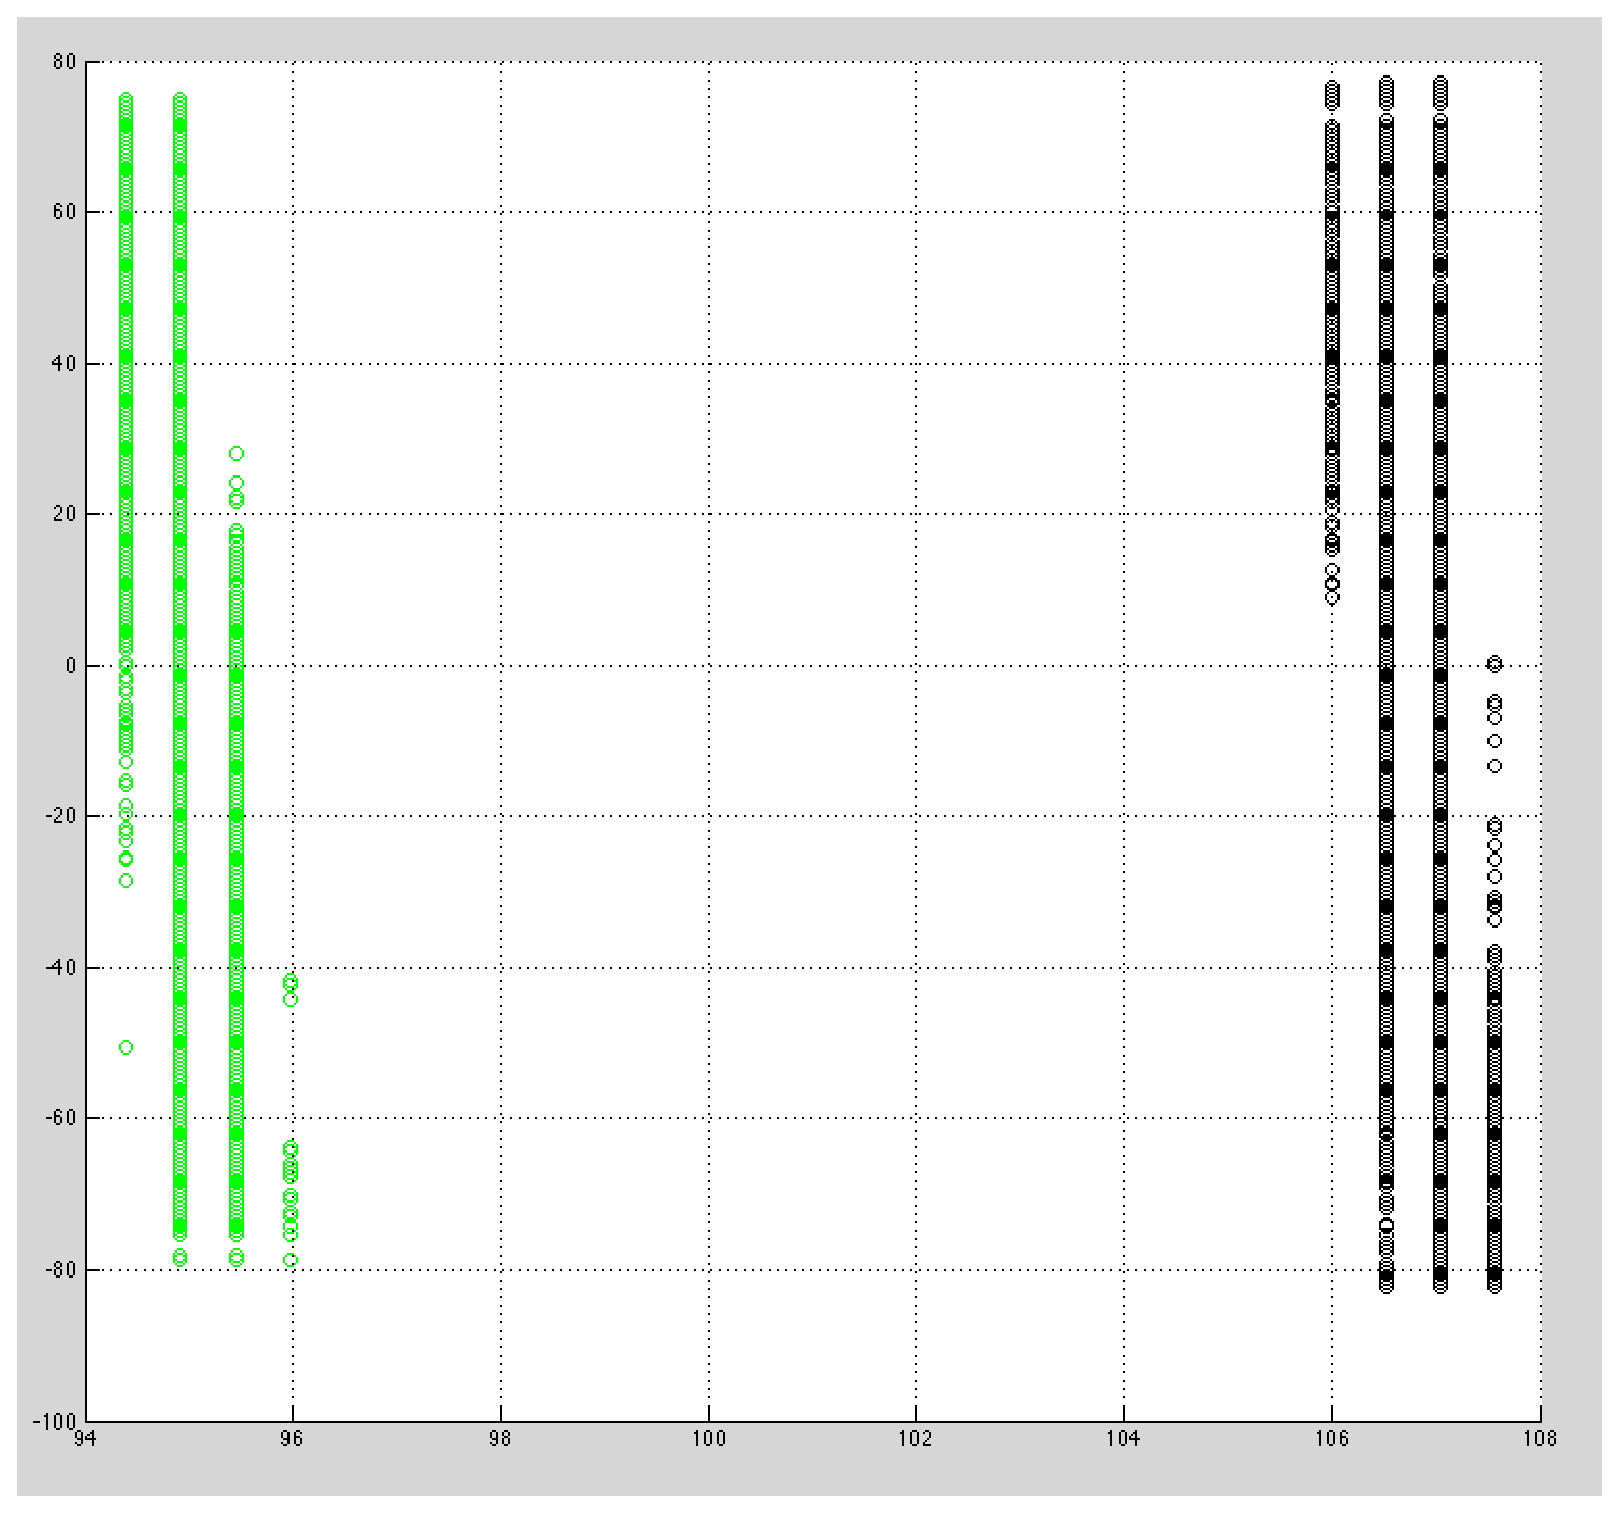
\includegraphics[width=2.75in]{data_extraction/images/surface_plane/inferior_comparison/Surface3_4.eps}}}
    \centerline{\emph{(b)}}
  \end{minipage}
  \begin{minipage}[t]{2.75in}
    \centering
    \centerline{\mbox{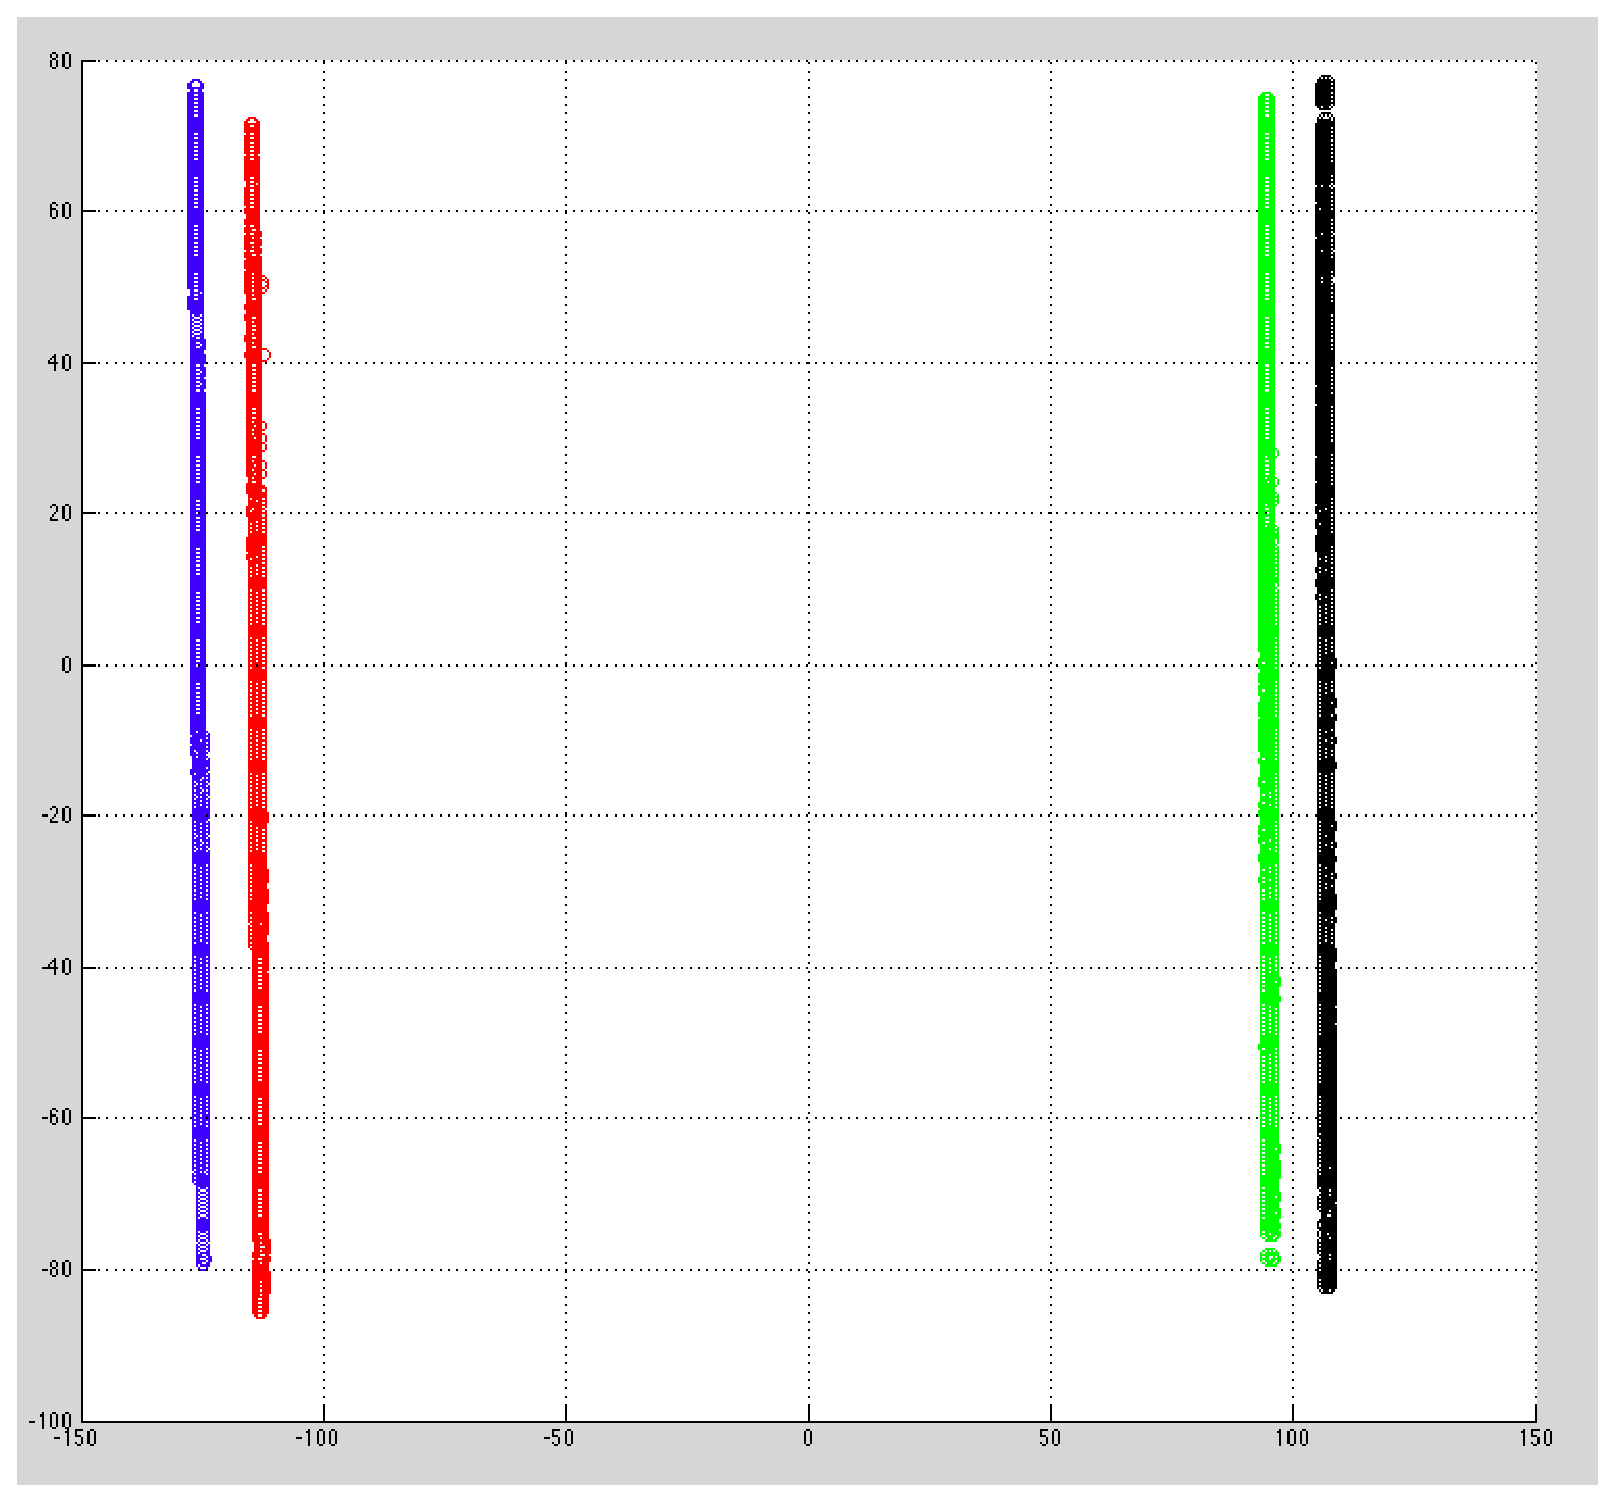
\includegraphics[width=2.75in]{data_extraction/images/surface_plane/Surface1_2_3_4.eps}}}
    \centerline{\emph{(c)}}
  \end{minipage}\medskip
  \begin{minipage}[t]{2.75in}
    \centering
    \centerline{\mbox{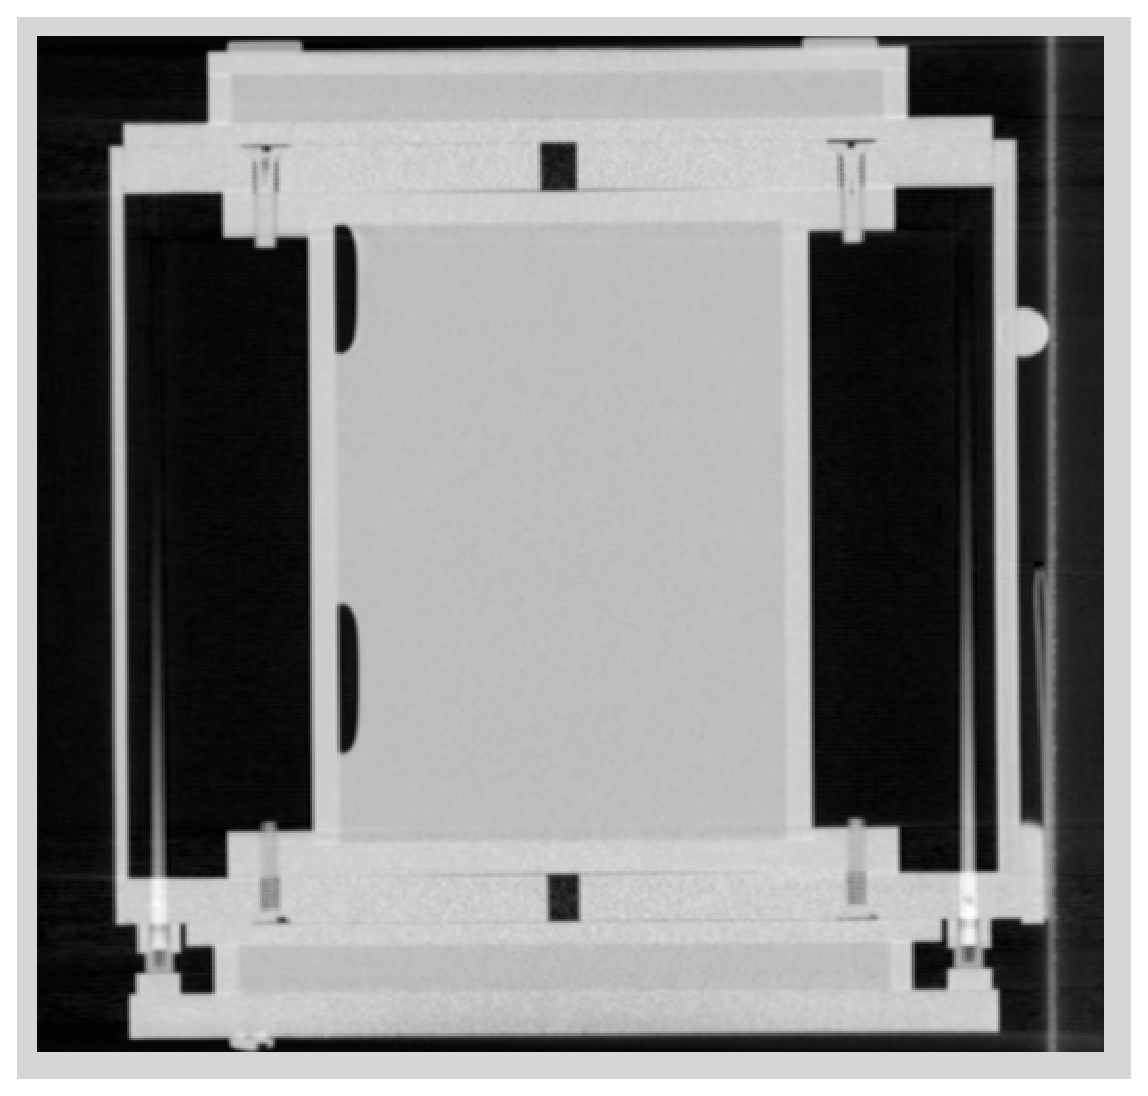
\includegraphics[width=2.75in]{data_extraction/images/surface_plane/saggital_ct_tilt.eps}}}
    \centerline{\emph{(d)}}
  \end{minipage}
  
  \caption{\emph{Water tank surfaces reconstruction from CT scan, YZ view}}
  \label{fig:ct_tank_surface_reconstruction_yz}

\end{figure}

\begin{figure}[htb]
  \begin{minipage}[t]{2.75in}
    \centering
    \centerline{\mbox{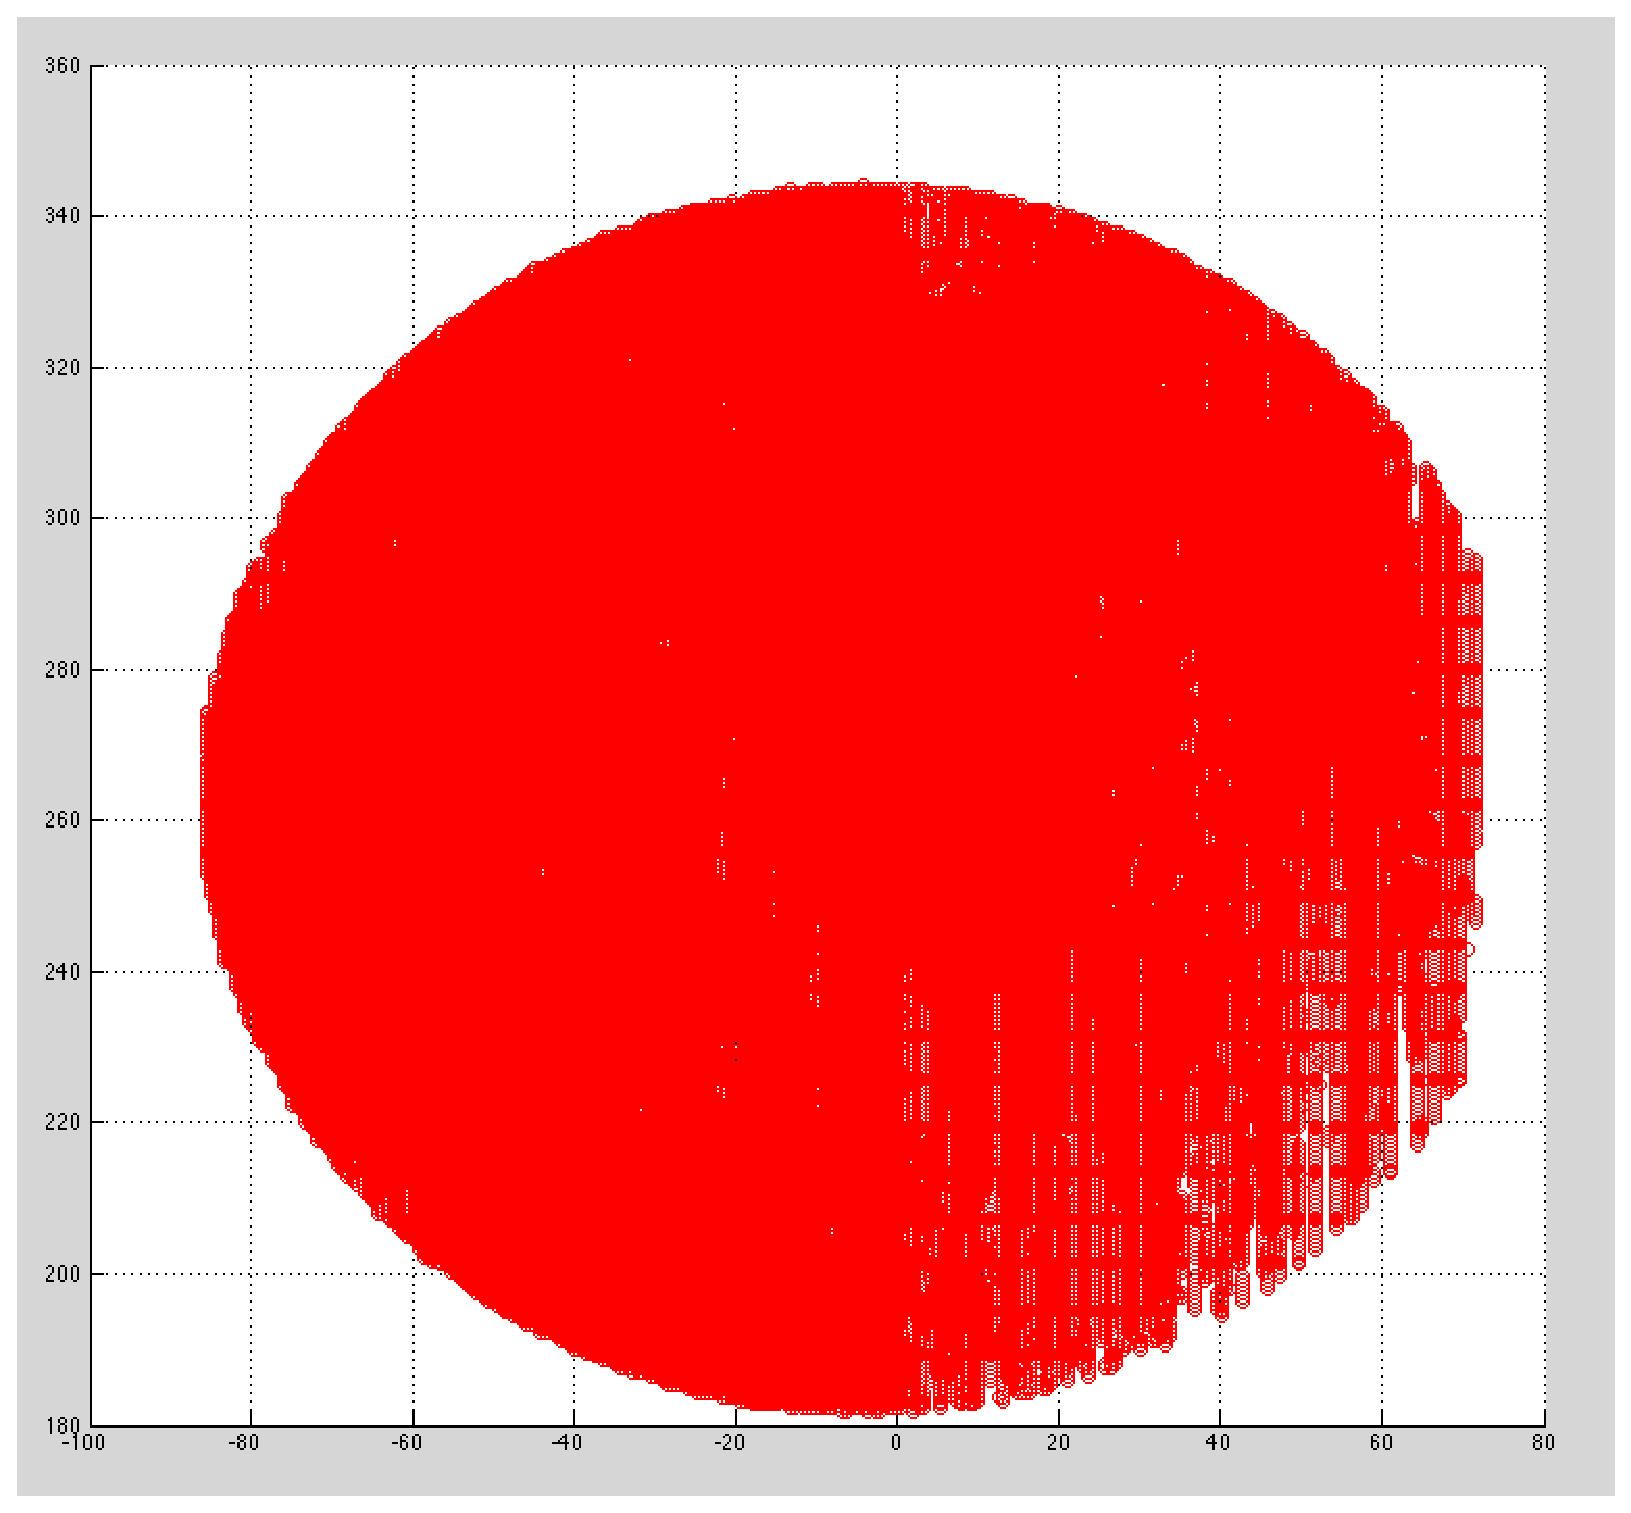
\includegraphics[width=2.75in]{data_extraction/images/surface_plane/superior_inside/xy.eps}}}
    \centerline{\emph{(a)}}
  \end{minipage}\medskip
  \begin{minipage}[t]{2.75in}
    \centering
    \centerline{\mbox{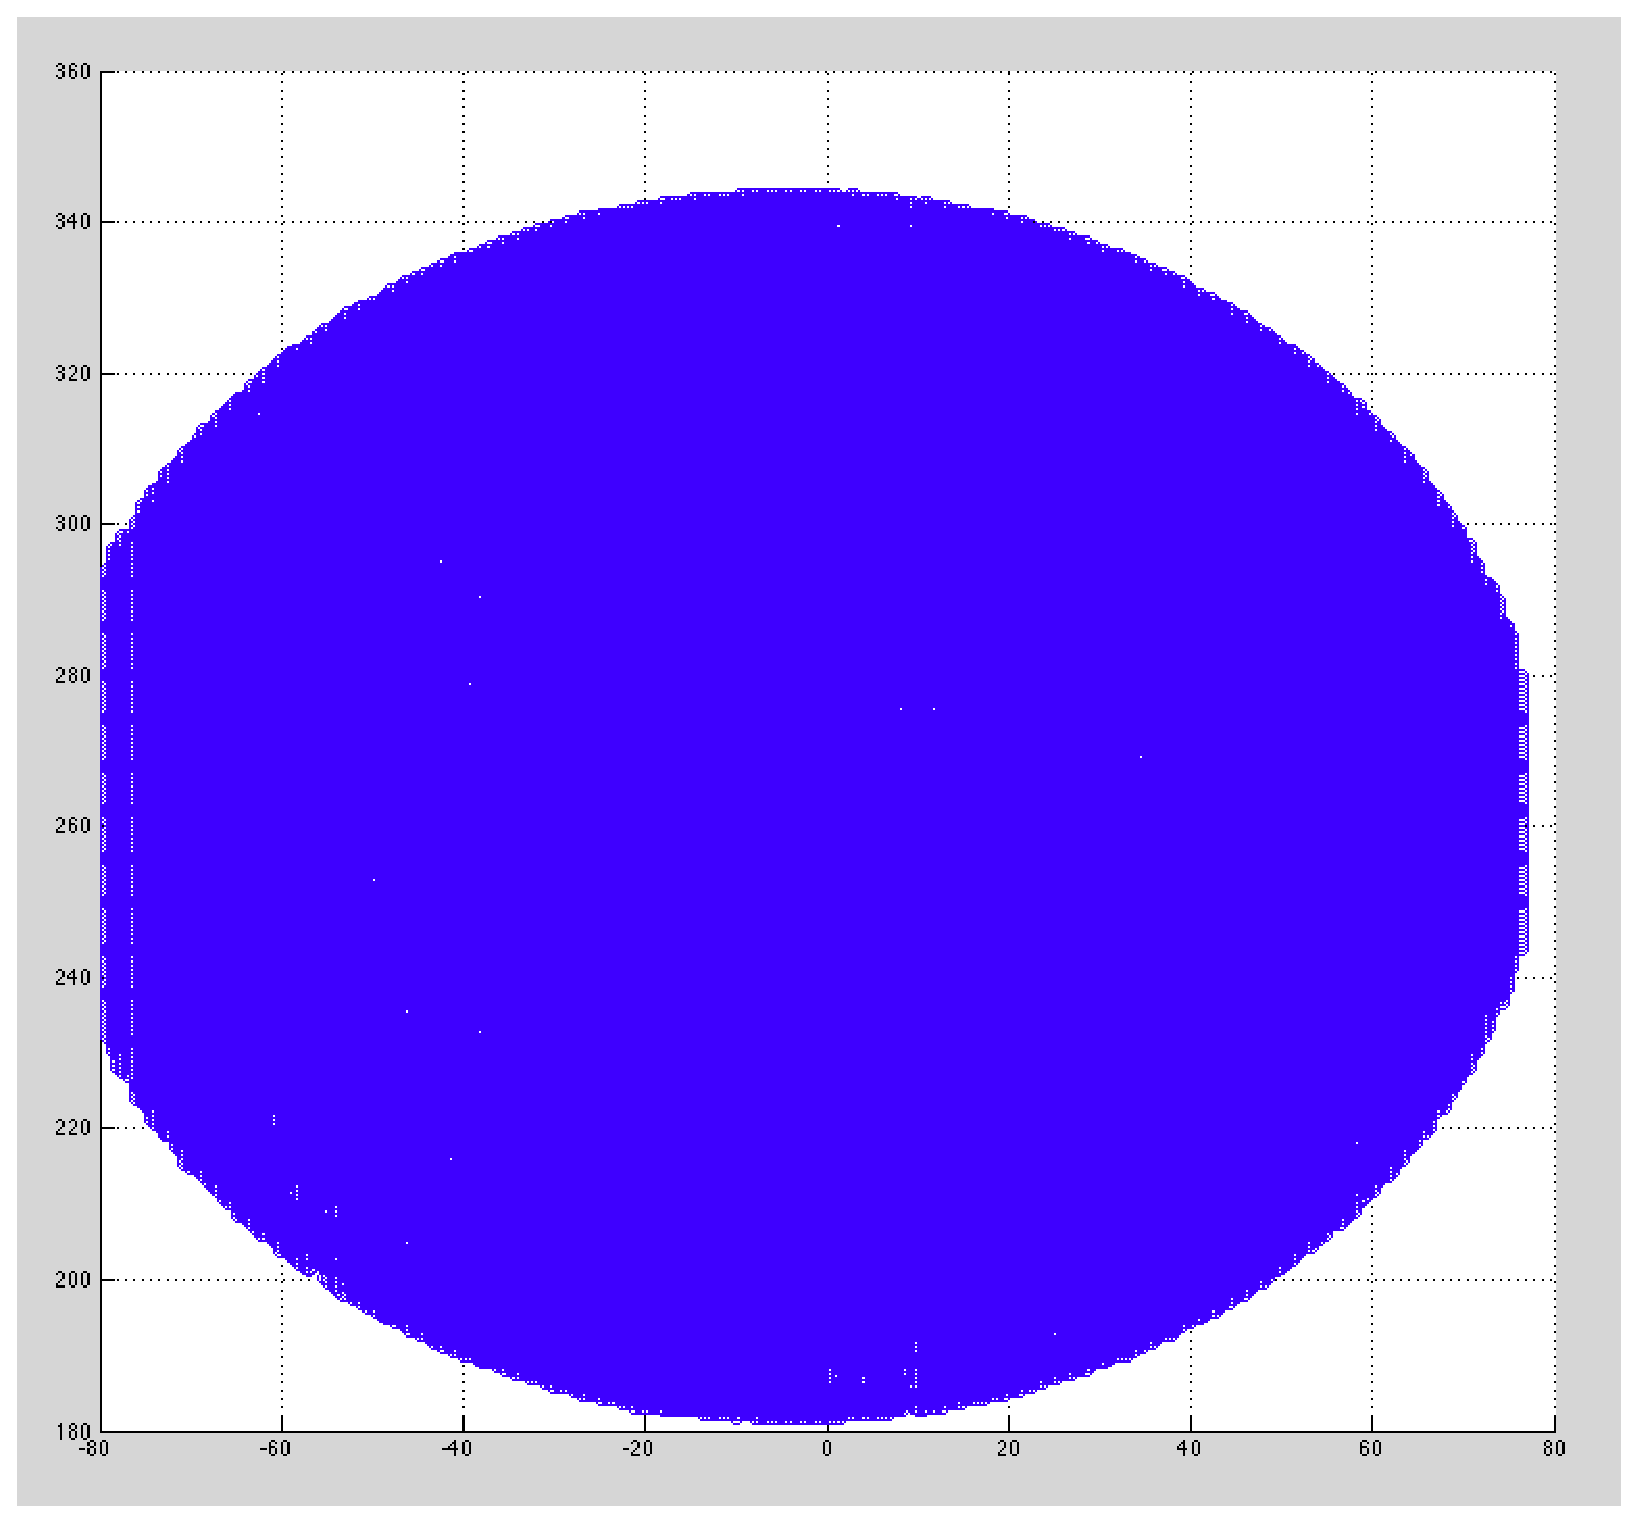
\includegraphics[width=2.75in]{data_extraction/images/surface_plane/superior_outside/xy.eps}}}
    \centerline{\emph{(b)}}
  \end{minipage}
  \begin{minipage}[t]{2.75in}
    \centering
    \centerline{\mbox{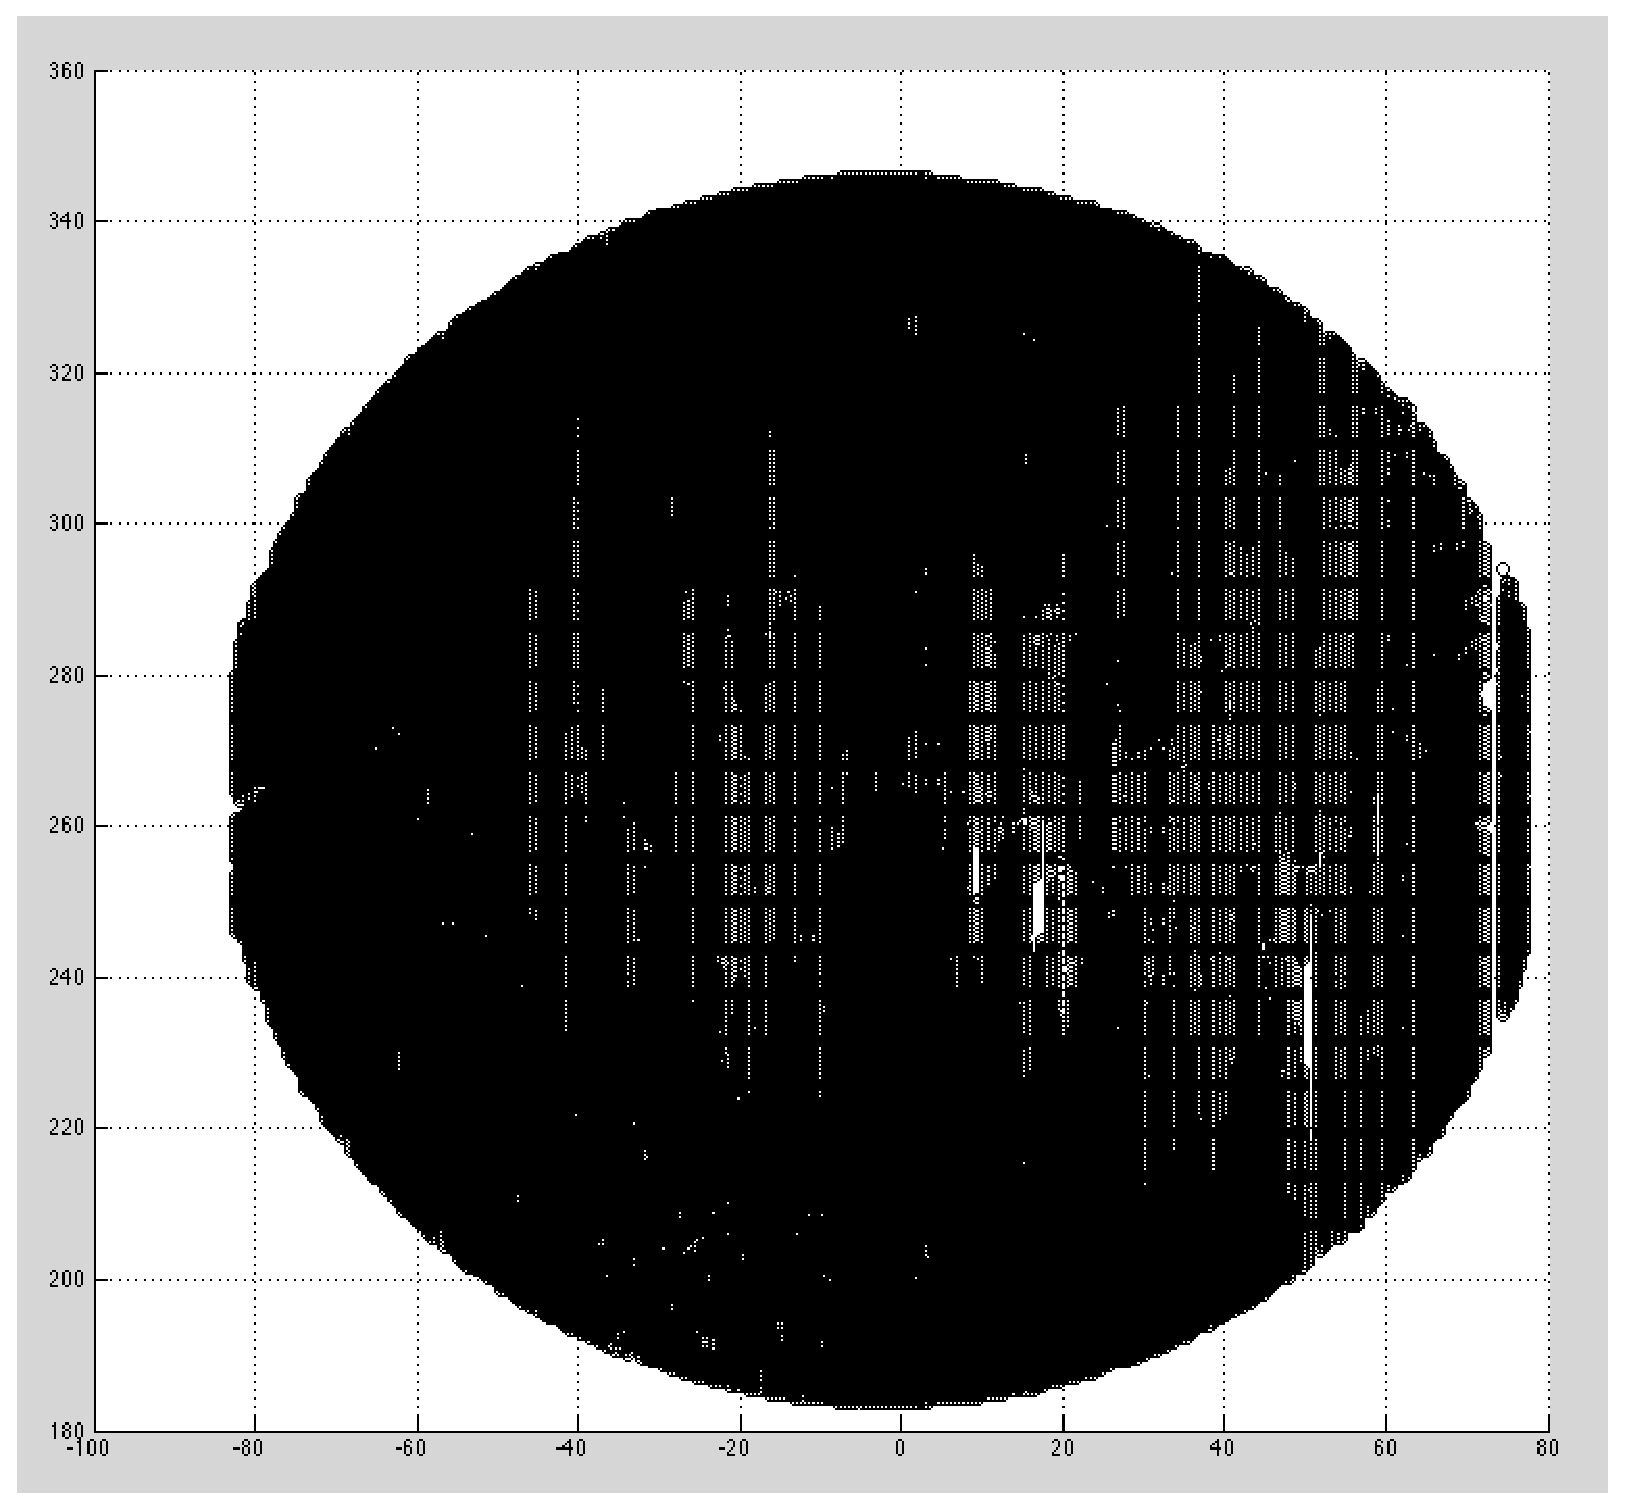
\includegraphics[width=2.75in]{data_extraction/images/surface_plane/inferior_inside/xy.eps}}}
    \centerline{\emph{(c)}}
  \end{minipage}\medskip
  \begin{minipage}[t]{2.75in}
    \centering
    \centerline{\mbox{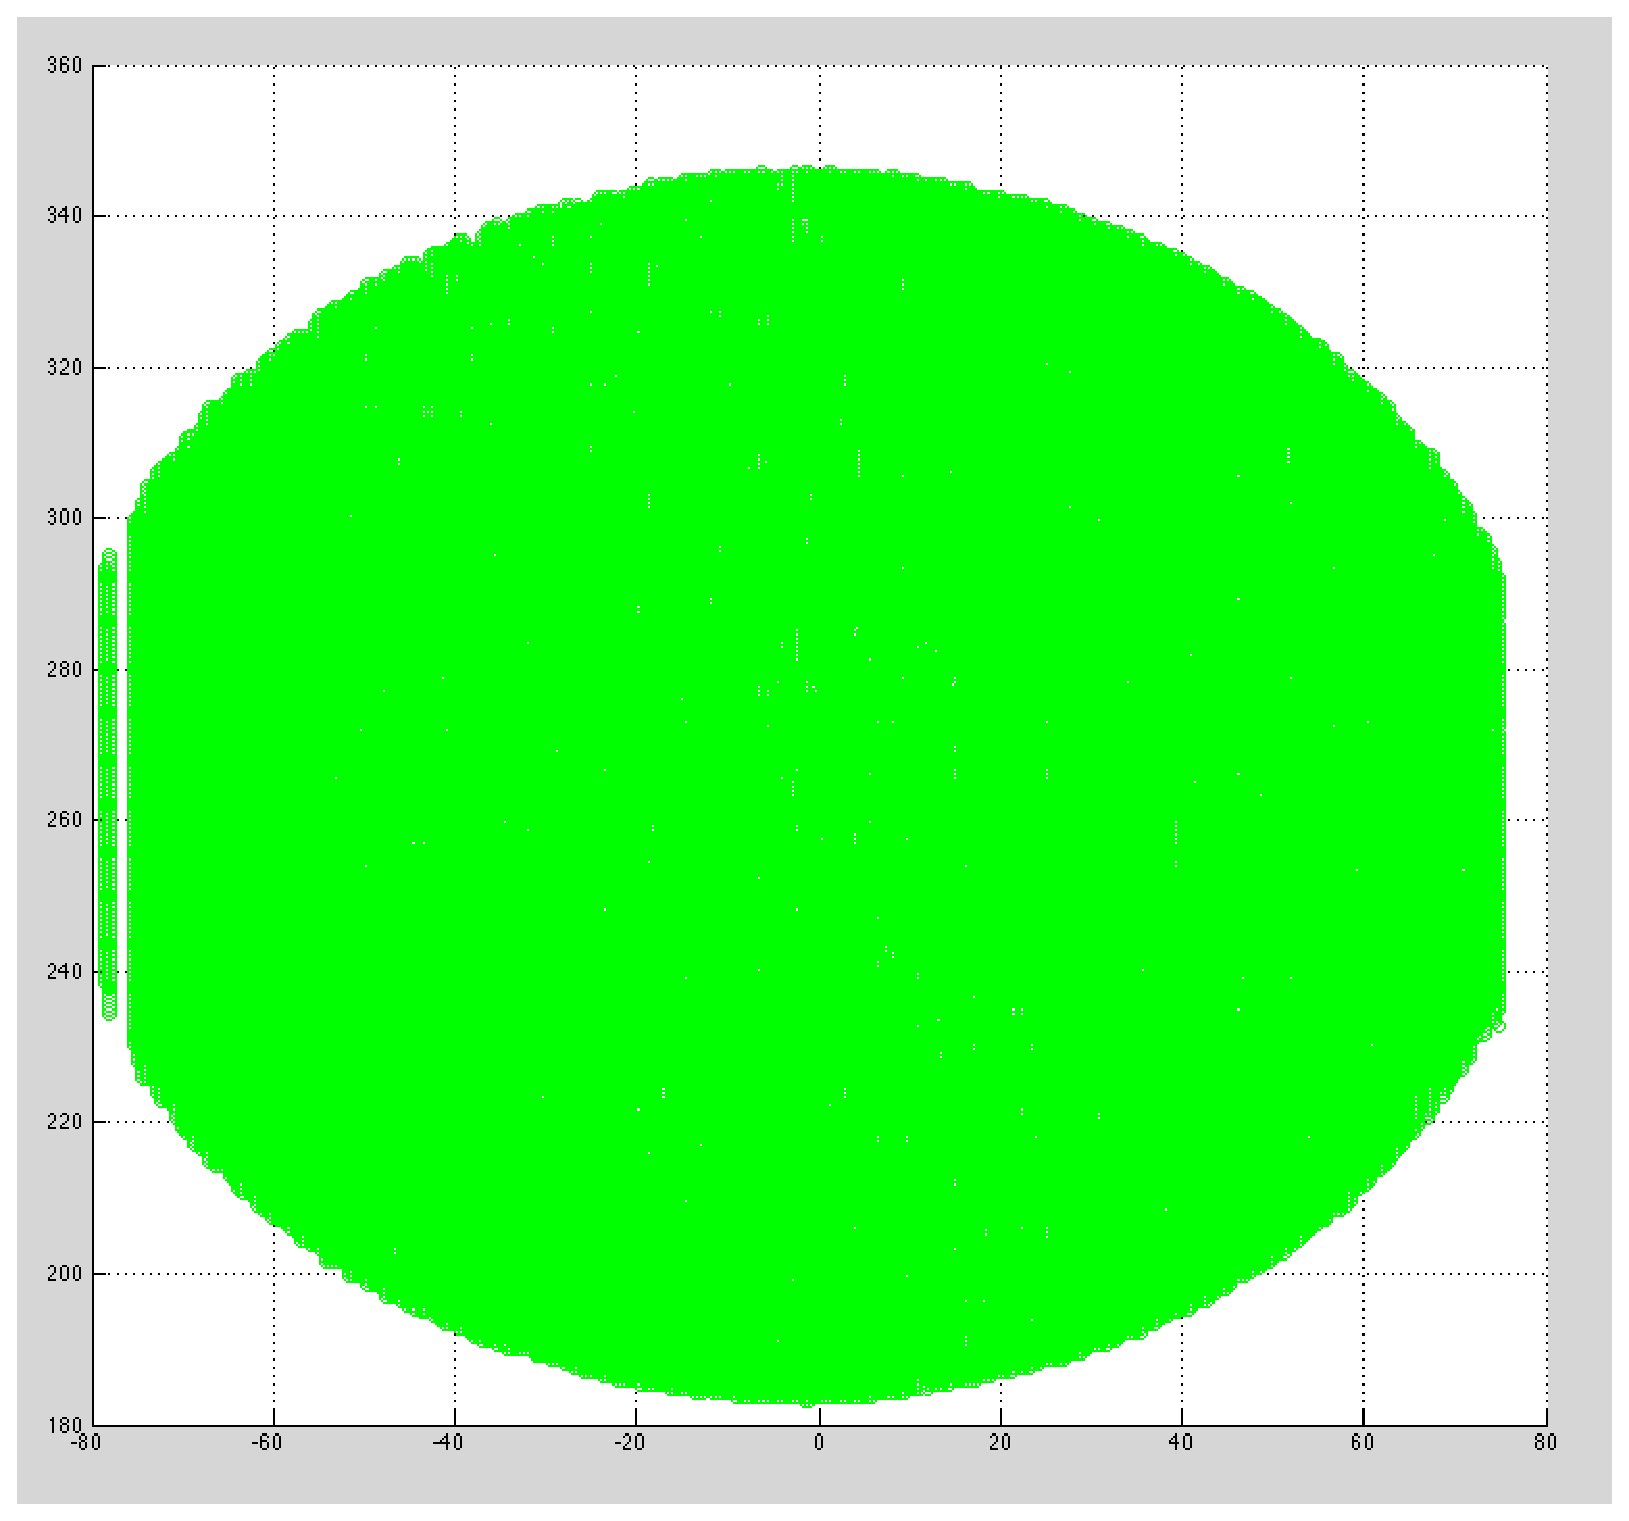
\includegraphics[width=2.75in]{data_extraction/images/surface_plane/inferior_outside/xy.eps}}}
    \centerline{\emph{(d)}}
  \end{minipage}
  \caption{\emph{Water tank surfaces reconstruction from CT scan, XY view}}
  \label{fig:ct_tank_surface_reconstruction_xy}
\end{figure}

Notice that in the YZ view in figure \ref{fig:ct_tank_surface_reconstruction_yz}(a) (b) (c), 
all four surfaces are tilted. This is consistant with what we observed on saggital reconstruction 
of this image set. 

\subsection{Estimating Surfaces Distances}


\section{Water Tank MRI}
\label{mri_tank}

\subsection{Introduction}
Naturally due to the similarity of MR image and CT images, one can imagine that we shall reuse the algorithm
we used to estimate water tank surfaces in CT images in MR images. However there are following challanges:
\begin{enumerage}
  \item MR images' quality is not as good as CT images. Espeically the water tank appeared at lower portion
    of images. That portion of the phantom is not completely inside the head coil, so the signals from that
    portion of the phantom contains a lot of noises. With that amount of noises, algorithm we used in CT 
    images tends to get incorrect results. % NOTES: Elaborate or add examples 
  \item Unlike CT images, which has no distortion in the images, MR images are distorted. Tank surfaces
    in MR images have curvature. So when processing the curvatured noisy edge, we can't really use straight
    line anymore, there has to be another reliable way to help us trace the broken, noisy curved edges.
  \item Because CT images are not distorted, missing some data points at the edges is not that important.
    With most data we collected, we can still construct a pretty accurate surfaces. However, since MR images
    are distorted, data points on the edges are especially important because they contain the most information
    about the distortion model.
\end{enumerate}

Once apprach is to use 

Different cases:
\begin{itemize}
\item Top surface: remove robber pads
\item bottom surface: noise
\item Slices toward the edge % THOUGHT: we could probably combine both saggital and coronal reconstruction to collect a more complete data points
\end{itemize}

NOTE: old get_horizontal_boundaries is obvious not as sophisticated as the newer one, it would not even handle
the mid slice well.

horizontal boundaries for surfaces:
\begin{enumerate}
\item Locate tube regions on either side of the water tank
\item First we need to start from the middle to get an accurate middle slice's left and right boundary. To
  do this we will average middle slice and it's previous and next images to get rid of some of noise signals 
  as well as enhance the real data signals. 
\item We will use both coronal and saggital set to extract surfaces
\item Bottom tank's boundaries could just use the upper tank's
\item Only the exterior inside surface will use canny for edges, every other surface will use column wised
  data analysis. 
  All surfaces will use the same left and right boundaries derived from exterior inside surface.
  Column wised pixel analysis should be able distinguish padding region and columns that might be outside
  left or right boundaries.
\item Averging three slices work well for most of the slices. Experiments have shown that 60\% mid slices 
  is a good cut off point
\end{enumerate}
